\documentclass[hidelinks,12pt,a4paper]{article}
\usepackage[italian]{babel}
\usepackage[utf8]{inputenc}
\usepackage{fourier} 

% Images
\usepackage{graphicx}
\usepackage{caption}
\usepackage{subcaption}
\usepackage{float}
\graphicspath{ {../Images} }

% Stop hyphenation
\usepackage[none]{hyphenat}

% Dotted frame.
\usepackage{tikz}

% Adjust paragraph.
\usepackage{changepage}

% Coloring links
\usepackage{xcolor}

% License
\usepackage[
type={CC},
modifier={by-nc-sa},
version={4.0},
]{doclicense}

\begin{document}
	
	\title{\textbf{\centering{Laboratorio creativo per bambini}\\Collega le immagini alla descrizione}}
	\author{Alice Balestieri\\Francesco Rombaldoni}
	\date{}
	
	\maketitle
	\newpage
	
	\tableofcontents
	\newpage
	
	\section{Come giocare}
	\begin{center}
		\textbf{Le regole sono rivolte agli operatori.}
	\end{center}
	
	\subsection{Variante 1}
	 Dopo aver ritagliato le immagini e le descrizioni (presenti nella sezione successiva), disporle casualmente su un tavolo. I bambini dovranno assegnare le immagini all'apposita descrizione sovrapponendole.\\
	Quando i bambini hanno completato l'associazione delle coppie, procedere alla correzione.
	
	\subsection{Variante 2}
	Dopo aver ritagliato le immagini e le descrizioni (presenti nella sezione successiva), disporre casualmente le immagini su un tavolo e mescolare le descrizioni depositando poi il mazzo in un angolo del tavolo.\\
	Dividere i bambini in squadre. A turno ogni squadra dovrà pescare una descrizione dal mazzo e accoppiare quest'ultima ad un'immagine presente sul tavolo.\\
	Si procede immediatamente alla correzione, qualora la coppia formata sia corretta, la squadra trattiene le carte e termina il turno. Nel caso in cui la coppia formata sia errata(evitando di lasciare intendere quale possa essere la soluzione), la squadra termina il turno. L'immagine viene riposizionata sul tavolo e la descrizione viene mescolata nuovamente all'interno del mazzo delle descrizioni.\\
	Quando le squadre dei bambini hanno finito di creare le coppie correttamente, la squadra che possiede nella propria mano il maggior numero di carte, vince la partita.
	
	\vspace*{\fill}
	\centering
	\fboxrule=2pt
	\fbox
	{
		\begin{minipage}{\linewidth}
			In caso di dubbi per la correzione, tenere una copia digitale di questo documento consultabile dallo "smartphone". Nella sezione "Immagini e descrizioni" ogni immagine è presentata con la relativa descrizione posta inferiormente.
		\end{minipage}
	 }
	
	\newpage
	\section{Immagini e descrizioni}
	
%-------- Starting images & descriptions section --------
	\begin{figure}[h]
			\centering
			\begin{tikzpicture}
				\node[draw,dashed]
				{
					\fboxrule=4pt			
					\fcolorbox{white}{white}{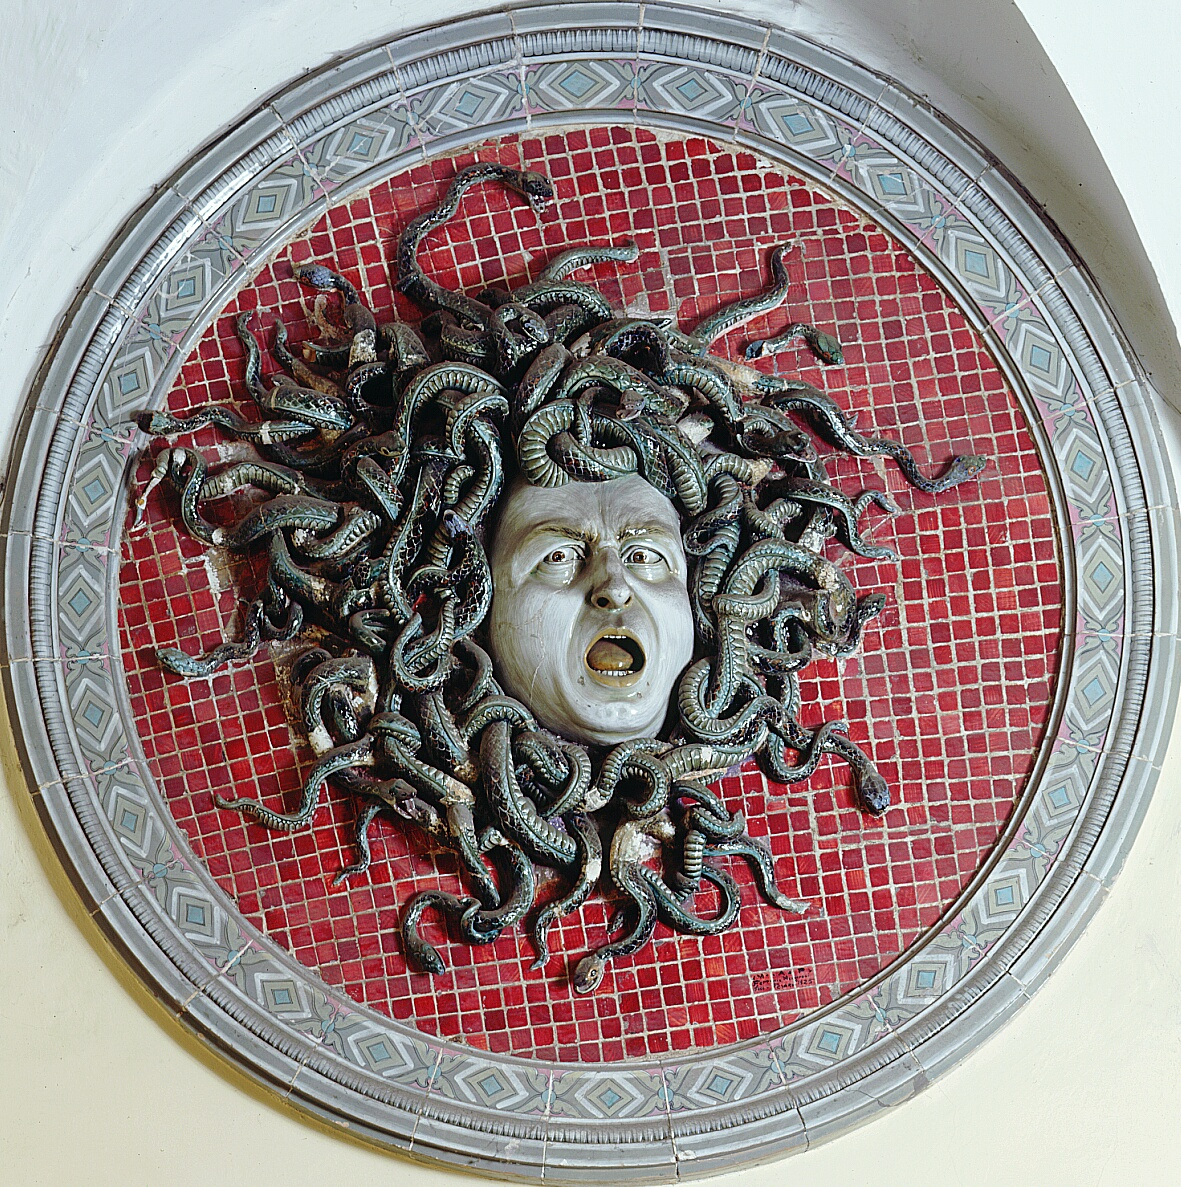
\includegraphics[scale=2]{Mengaroni_Ferruccio-Medusa.jpg}}
				};
			\end{tikzpicture}
	\end{figure}

	\begin{minipage}{\linewidth}
		\centering
		\begin{tikzpicture}
				\node[draw,dashed]
				{
					\fboxrule=4pt
					\fcolorbox{white}{white}{
						\fbox{
							\begin{minipage}{90mm}
								\raggedright
								{
									La testa della Medusa, circondata da innumerevoli serpi, raffigura il volto di Ferruccio Mengaroni. Il tondo ceramico è stato ispirato in parte dalle opere di Caravaggio e dal mito greco el mostro Medusa. Quest'opera è avvolta da una misteriosa maledizione e durante il suo trasporto alla Biennale di Arti decorative di Monza si sbilanciò e Ferruccio Mengaroni, temendo si rompesse, accorse a sorreggerla ma purtroppo venne schiacchiato dal peso del suo capolavoro.
								}
							\end{minipage}
						}
					}
				};
		\end{tikzpicture}
	\end{minipage}

	\newpage
	%-------- End image --------
	
	\begin{figure}[h]
		\centering
		\begin{tikzpicture}
			\node[draw,dashed]
			{
				\fboxrule=4pt			
				\fcolorbox{white}{white}{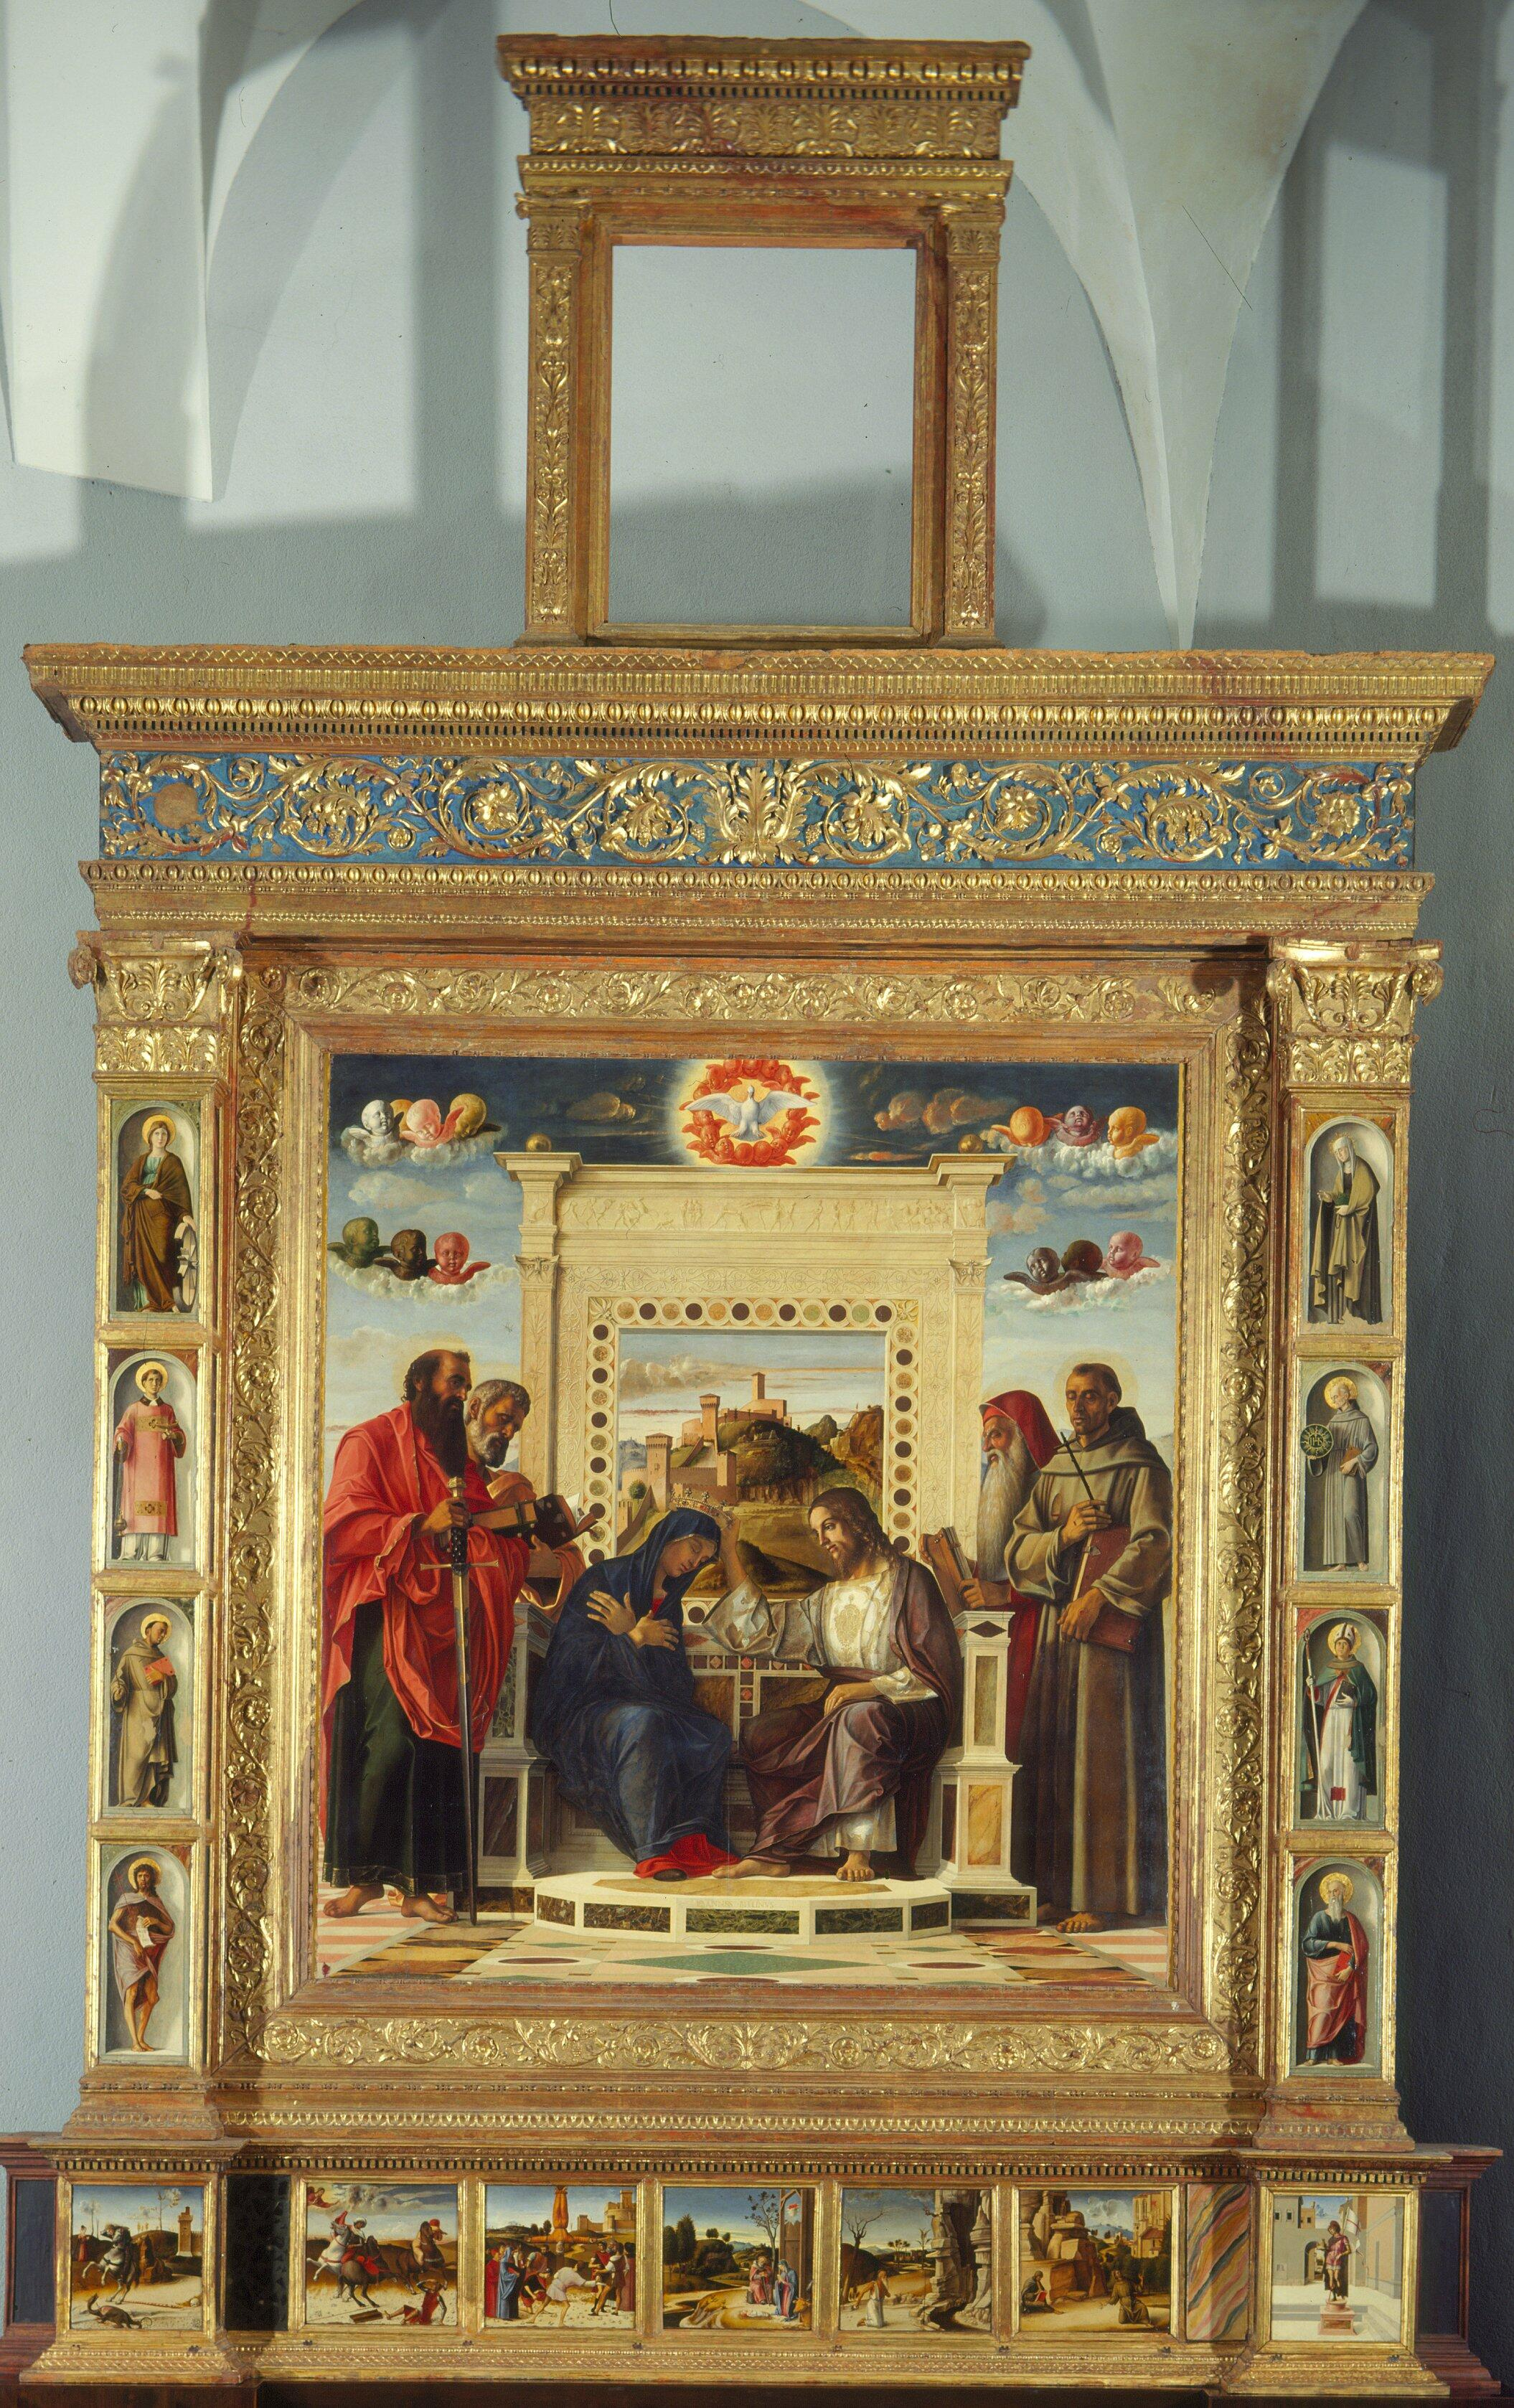
\includegraphics[scale=0.1]{Bellini_Giovanni-Incoronazione_della_Vergine.jpg}}
			};
		\end{tikzpicture}
	\end{figure}
	
	\begin{adjustwidth}{-30mm}{0mm}
		\begin{tikzpicture}
			\node[draw,dashed]
			{
				\fboxrule=4pt
				\fcolorbox{white}{white}{
					\fbox{
						\begin{minipage}{180mm}
							\raggedright
							{
								La Pala Bellini fu realizzata su commissione a Venezia dall'artista Giovanni Bellini per essere esposta all'interno della Chiesa di S. Francesco a Pesaro e venne trasportata via mare, divisa in parti e poi riassemblata in loco. Nel pannello centrale della pala è collocata la scena dell'Incoronazione della Vergine, che ha alle sue spalle, come sfondo, la celebre Rocca di Gradara mentre nella Predella (cornice) sono posti i Santi tra i quali S. Giorgio e il Drago.
							}
						\end{minipage}
					}
				}
			};
		\end{tikzpicture}
	\end{adjustwidth}

	\newpage
	%-------- End image --------	
	
	\begin{figure}[h]
		\centering
		\begin{tikzpicture}
			\node[draw,dashed]
			{
				\fboxrule=4pt			
				\fcolorbox{white}{white}{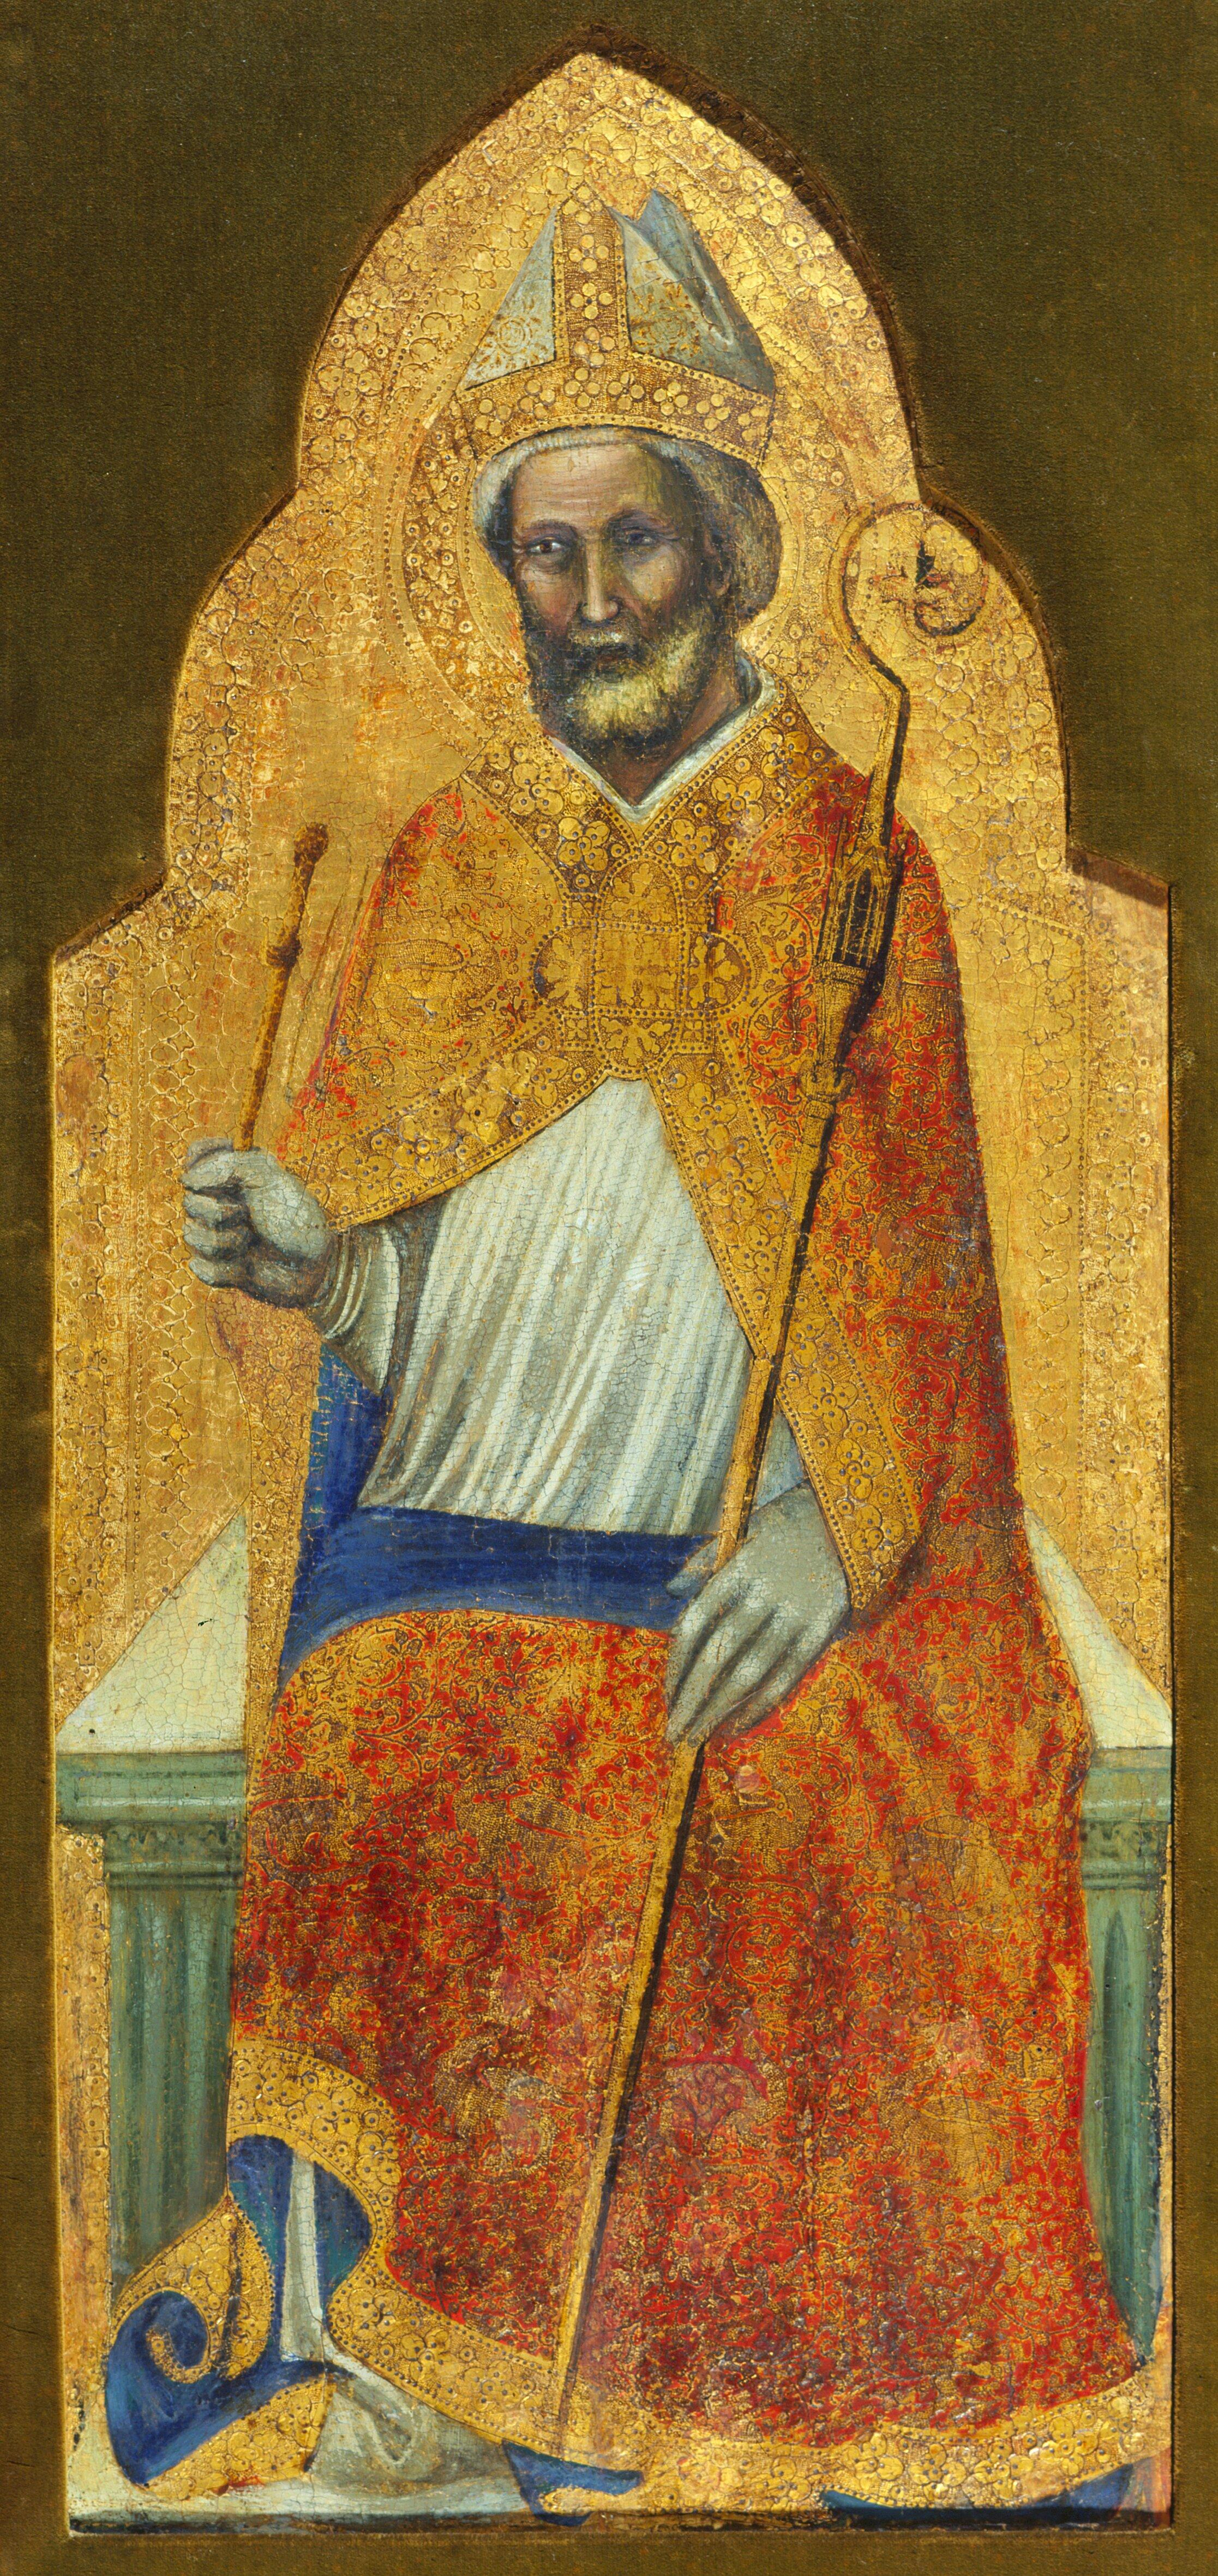
\includegraphics[scale=0.08]{Vitale_da_Bologna-Santo_Ambrogio_in_trono.jpg}}
			};
		\end{tikzpicture}
	\end{figure}
	
	\begin{minipage}{\linewidth}
		\centering
		\begin{tikzpicture}
			\node[draw,dashed]
			{
				\fboxrule=4pt
				\fcolorbox{white}{white}{
					\fbox{
						\begin{minipage}{70mm}
							\raggedright
							{
								La tavola raffigura un Santo Vescovo seduto, che impugna un bastone pastorale. Il quadro è privo di prospettiva, ma riccamente decorato in oro e per questo motivo fa parte della Collezione Rossini.
							}
						\end{minipage}
					}
				}
			};
		\end{tikzpicture}
	\end{minipage}
	
	\newpage
	%-------- End image --------
	
	\begin{figure}[h]
		\centering
		\begin{tikzpicture}
			\node[draw,dashed]
			{
				\fboxrule=4pt			
				\fcolorbox{white}{white}{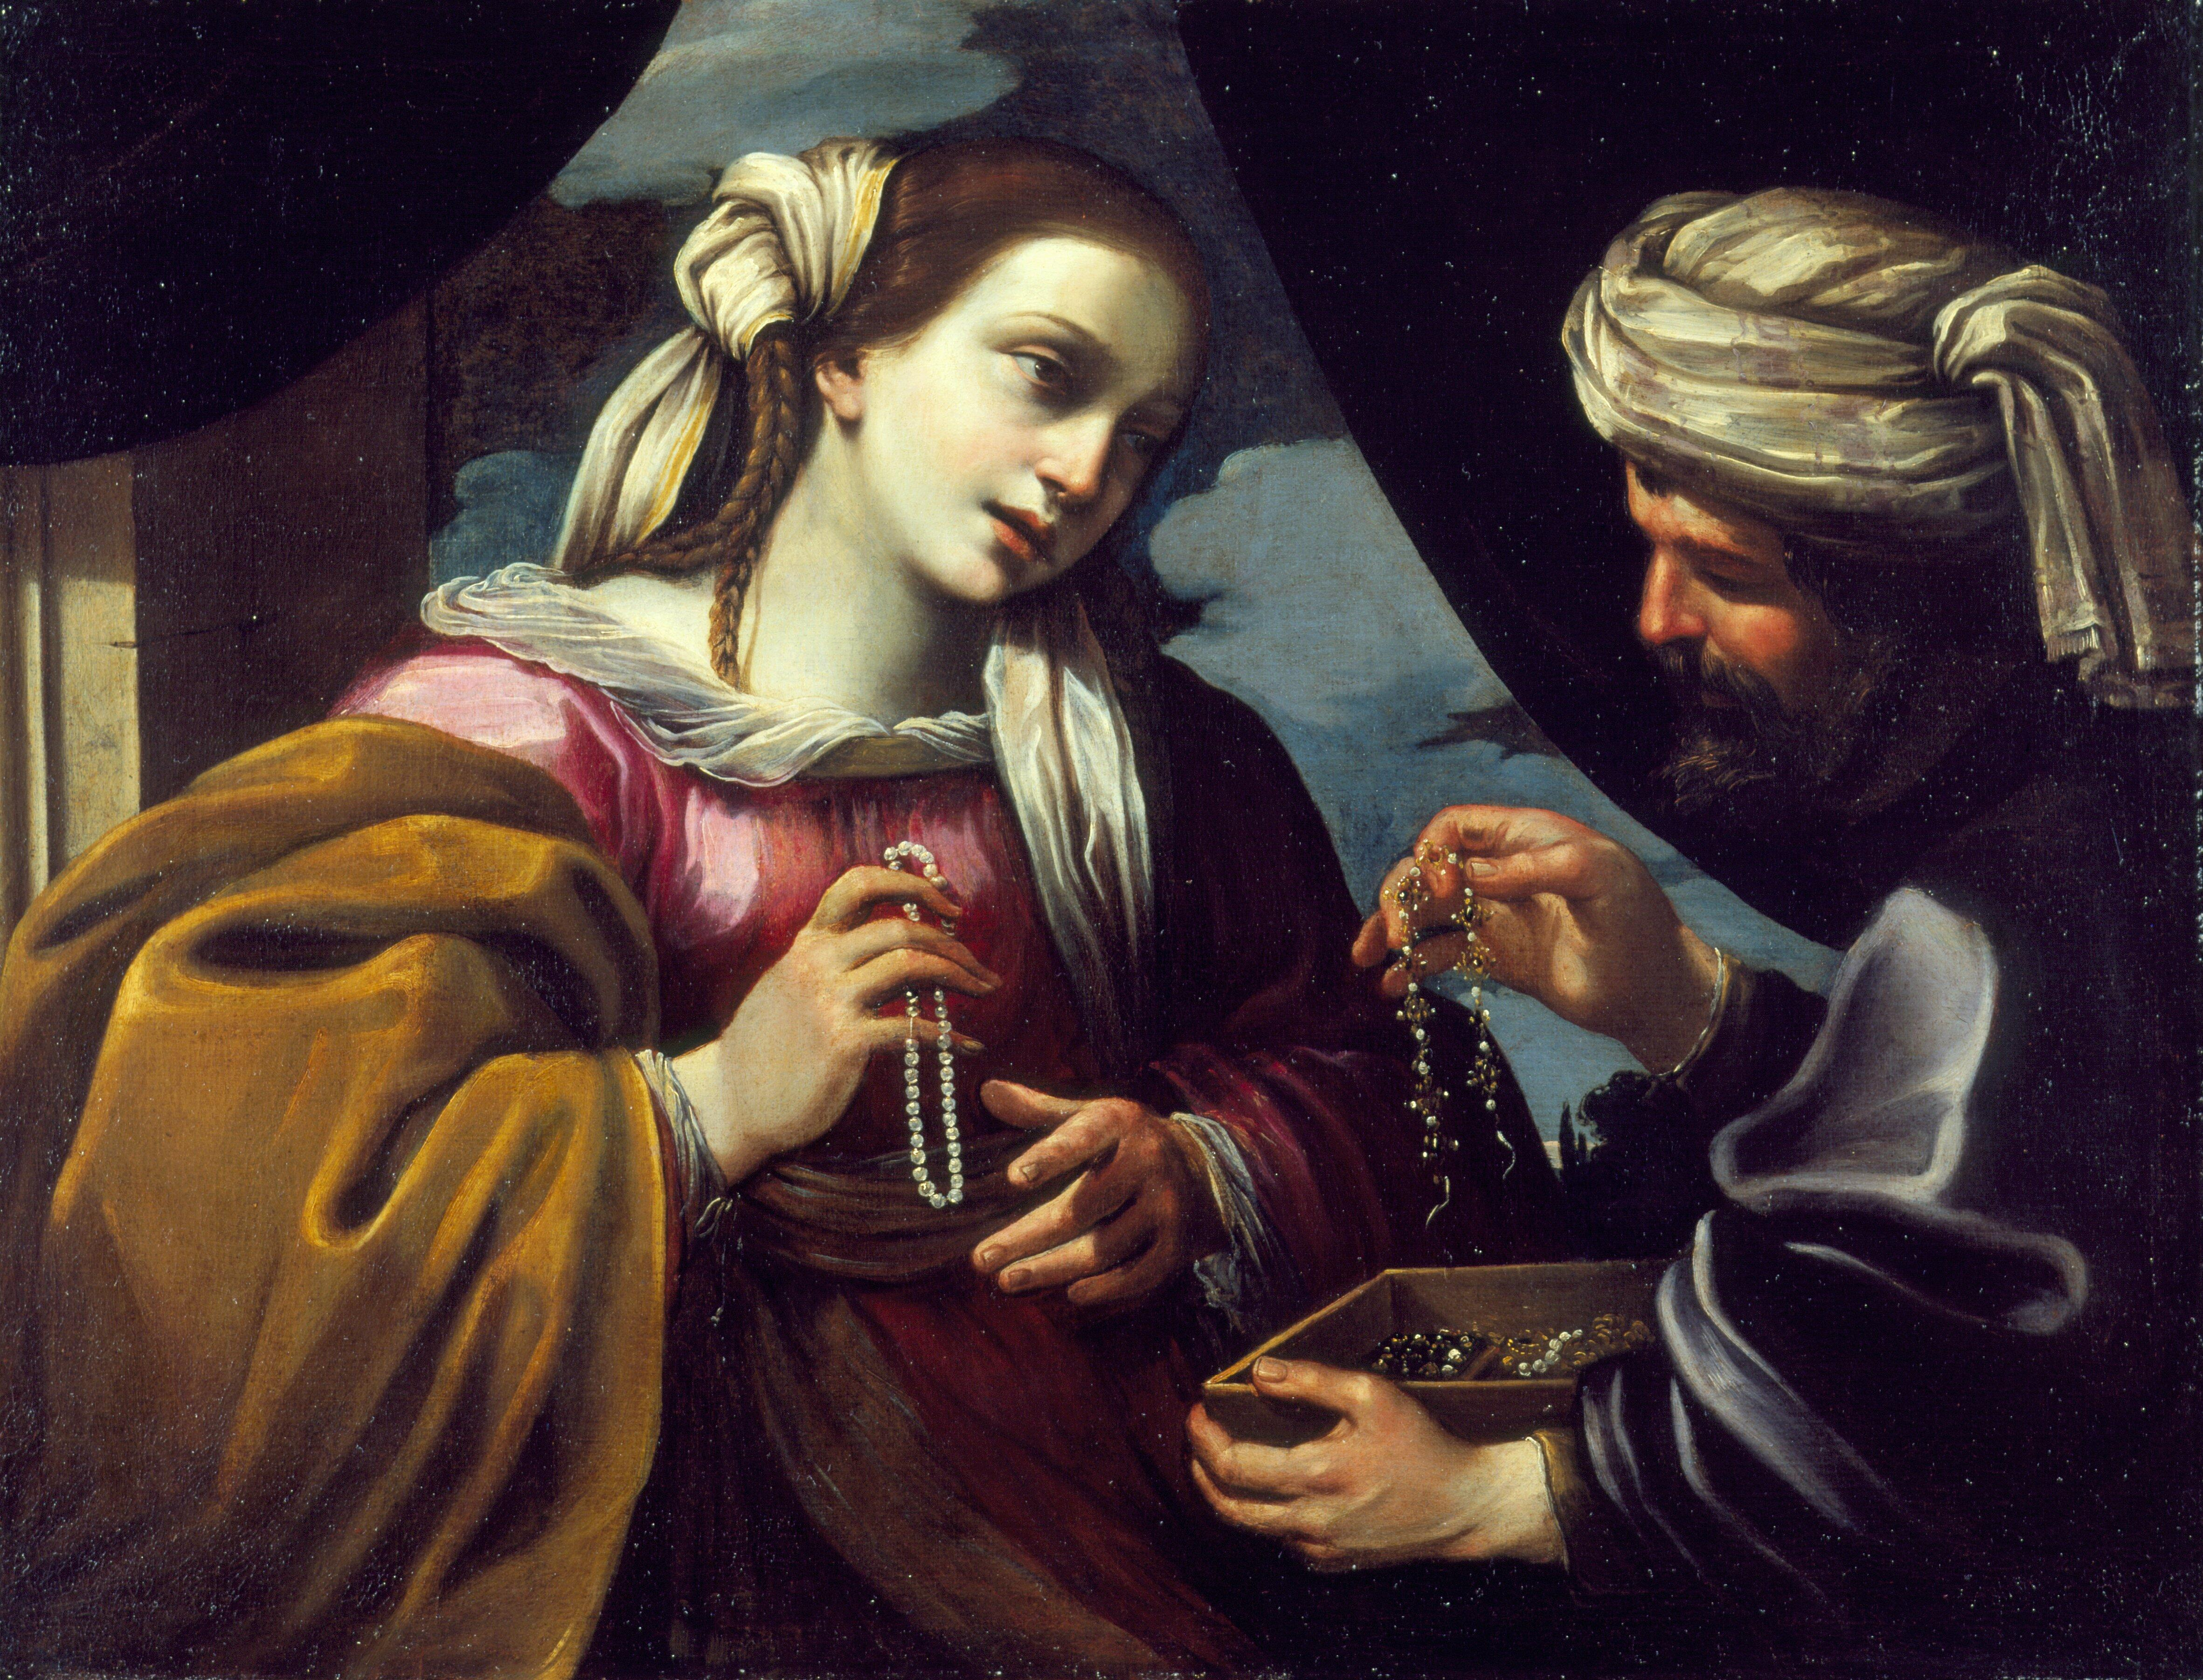
\includegraphics[scale = 0.08]{Desani_Pietro-Rebecca_ed_Eleazar.jpg}}
			};
		\end{tikzpicture}
	\end{figure}
	
	\begin{minipage}{\linewidth}
		\centering
		\begin{tikzpicture}
			\node[draw,dashed]
			{
				\fboxrule=4pt
				\fcolorbox{white}{white}{
					\fbox{
						\begin{minipage}{60mm}
							\raggedright
							{
								La tela raffigura Rebecca con una capigliatura a trecce e nastro. La donna ha in mano una collana di perle e sembra parlare con un uomo dal turbante annodato che solleva gioielli da una scatola.  
							}
						\end{minipage}
					}
				}
			};
		\end{tikzpicture}
	\end{minipage}
	
	\newpage
	%-------- End image --------
	
	\begin{figure}[h]
		\centering
		\begin{tikzpicture}
			\node[draw,dashed]
			{
				\fboxrule=4pt			
				\fcolorbox{white}{white}{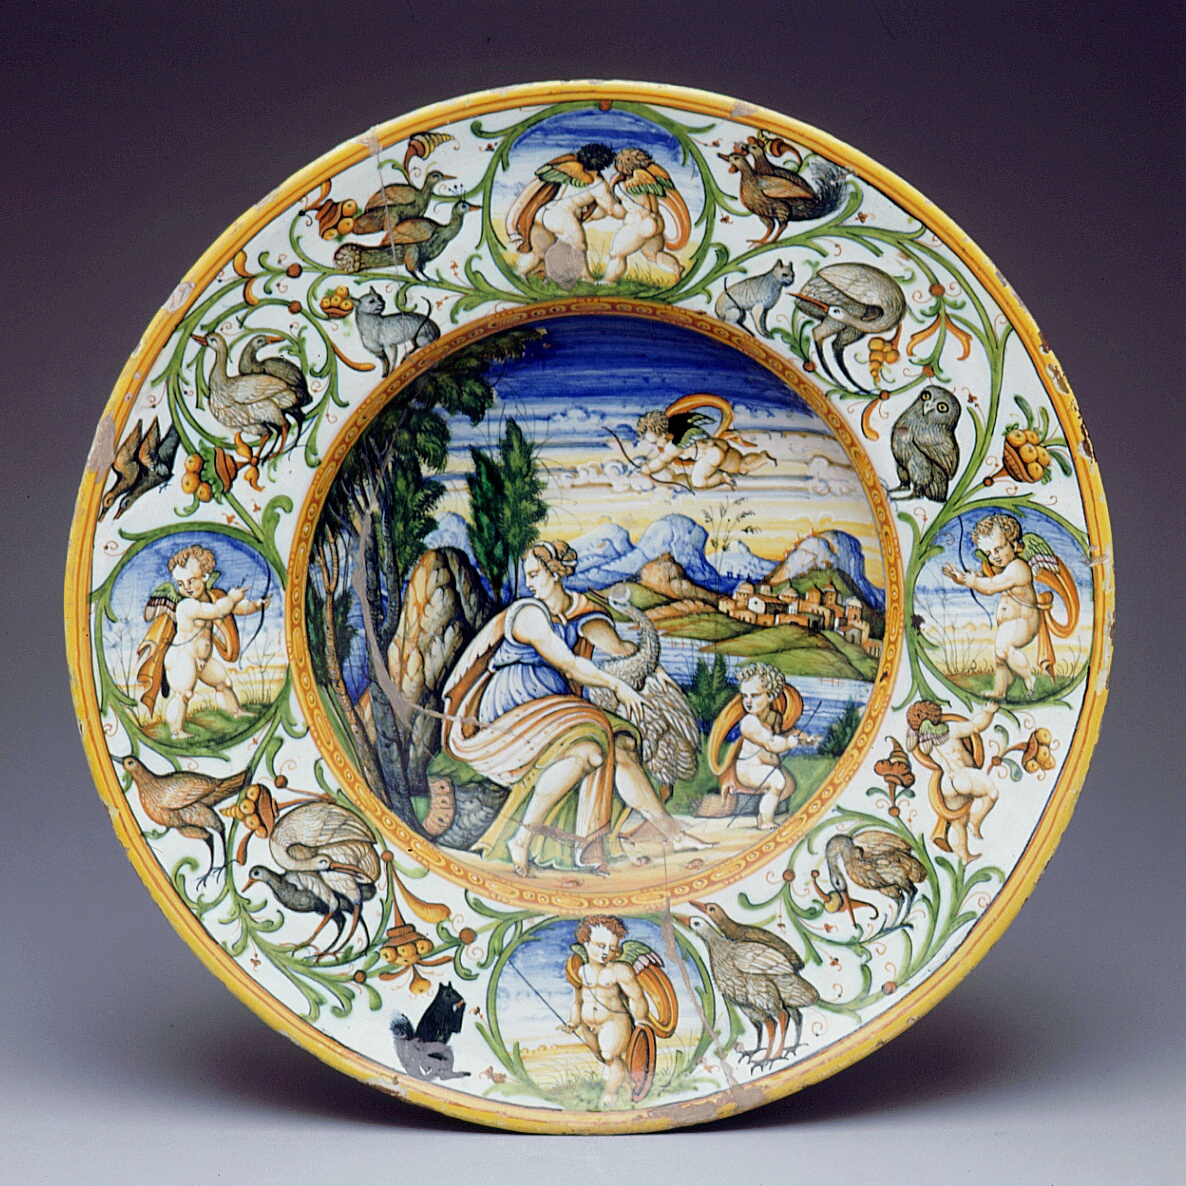
\includegraphics[scale = 1.8]{Giovanni_Antonio_Garella-Leda_e_il_cigno.jpg}}
			};
		\end{tikzpicture}
	\end{figure}
	
	\begin{minipage}{\linewidth}
		\centering
		\begin{tikzpicture}
			\node[draw,dashed]
			{
				\fboxrule=4pt
				\fcolorbox{white}{white}{
					\fbox{
						\begin{minipage}{70mm}
							\raggedright
							{
								Leda accarezza il cigno, nel quale si era mutato Giove per sedurla.\\
								Due cupidi, uno in basso accovacciato a sinistra, e uno in alto intento a scoccare una freccia, completano l'episodio.\\
								Sul fondo distese acquee, case addossate a collinette e vette montuose; sulla sinistra rocce e tre alberi, uno dei quali posto al limite del bordo. Sono raffigurati anche animali tra i quali uno scoiattolo dall'insolito colore nero come appariva 500 anni fa.\\
							
							}
						\end{minipage}
					}
				}
			};
		\end{tikzpicture}
	\end{minipage}
	
	\newpage
	%-------- End image --------
	
	\begin{figure}[h]
		\centering
		\begin{tikzpicture}
			\node[draw,dashed]
			{
				\fboxrule=4pt			
				\fcolorbox{white}{white}{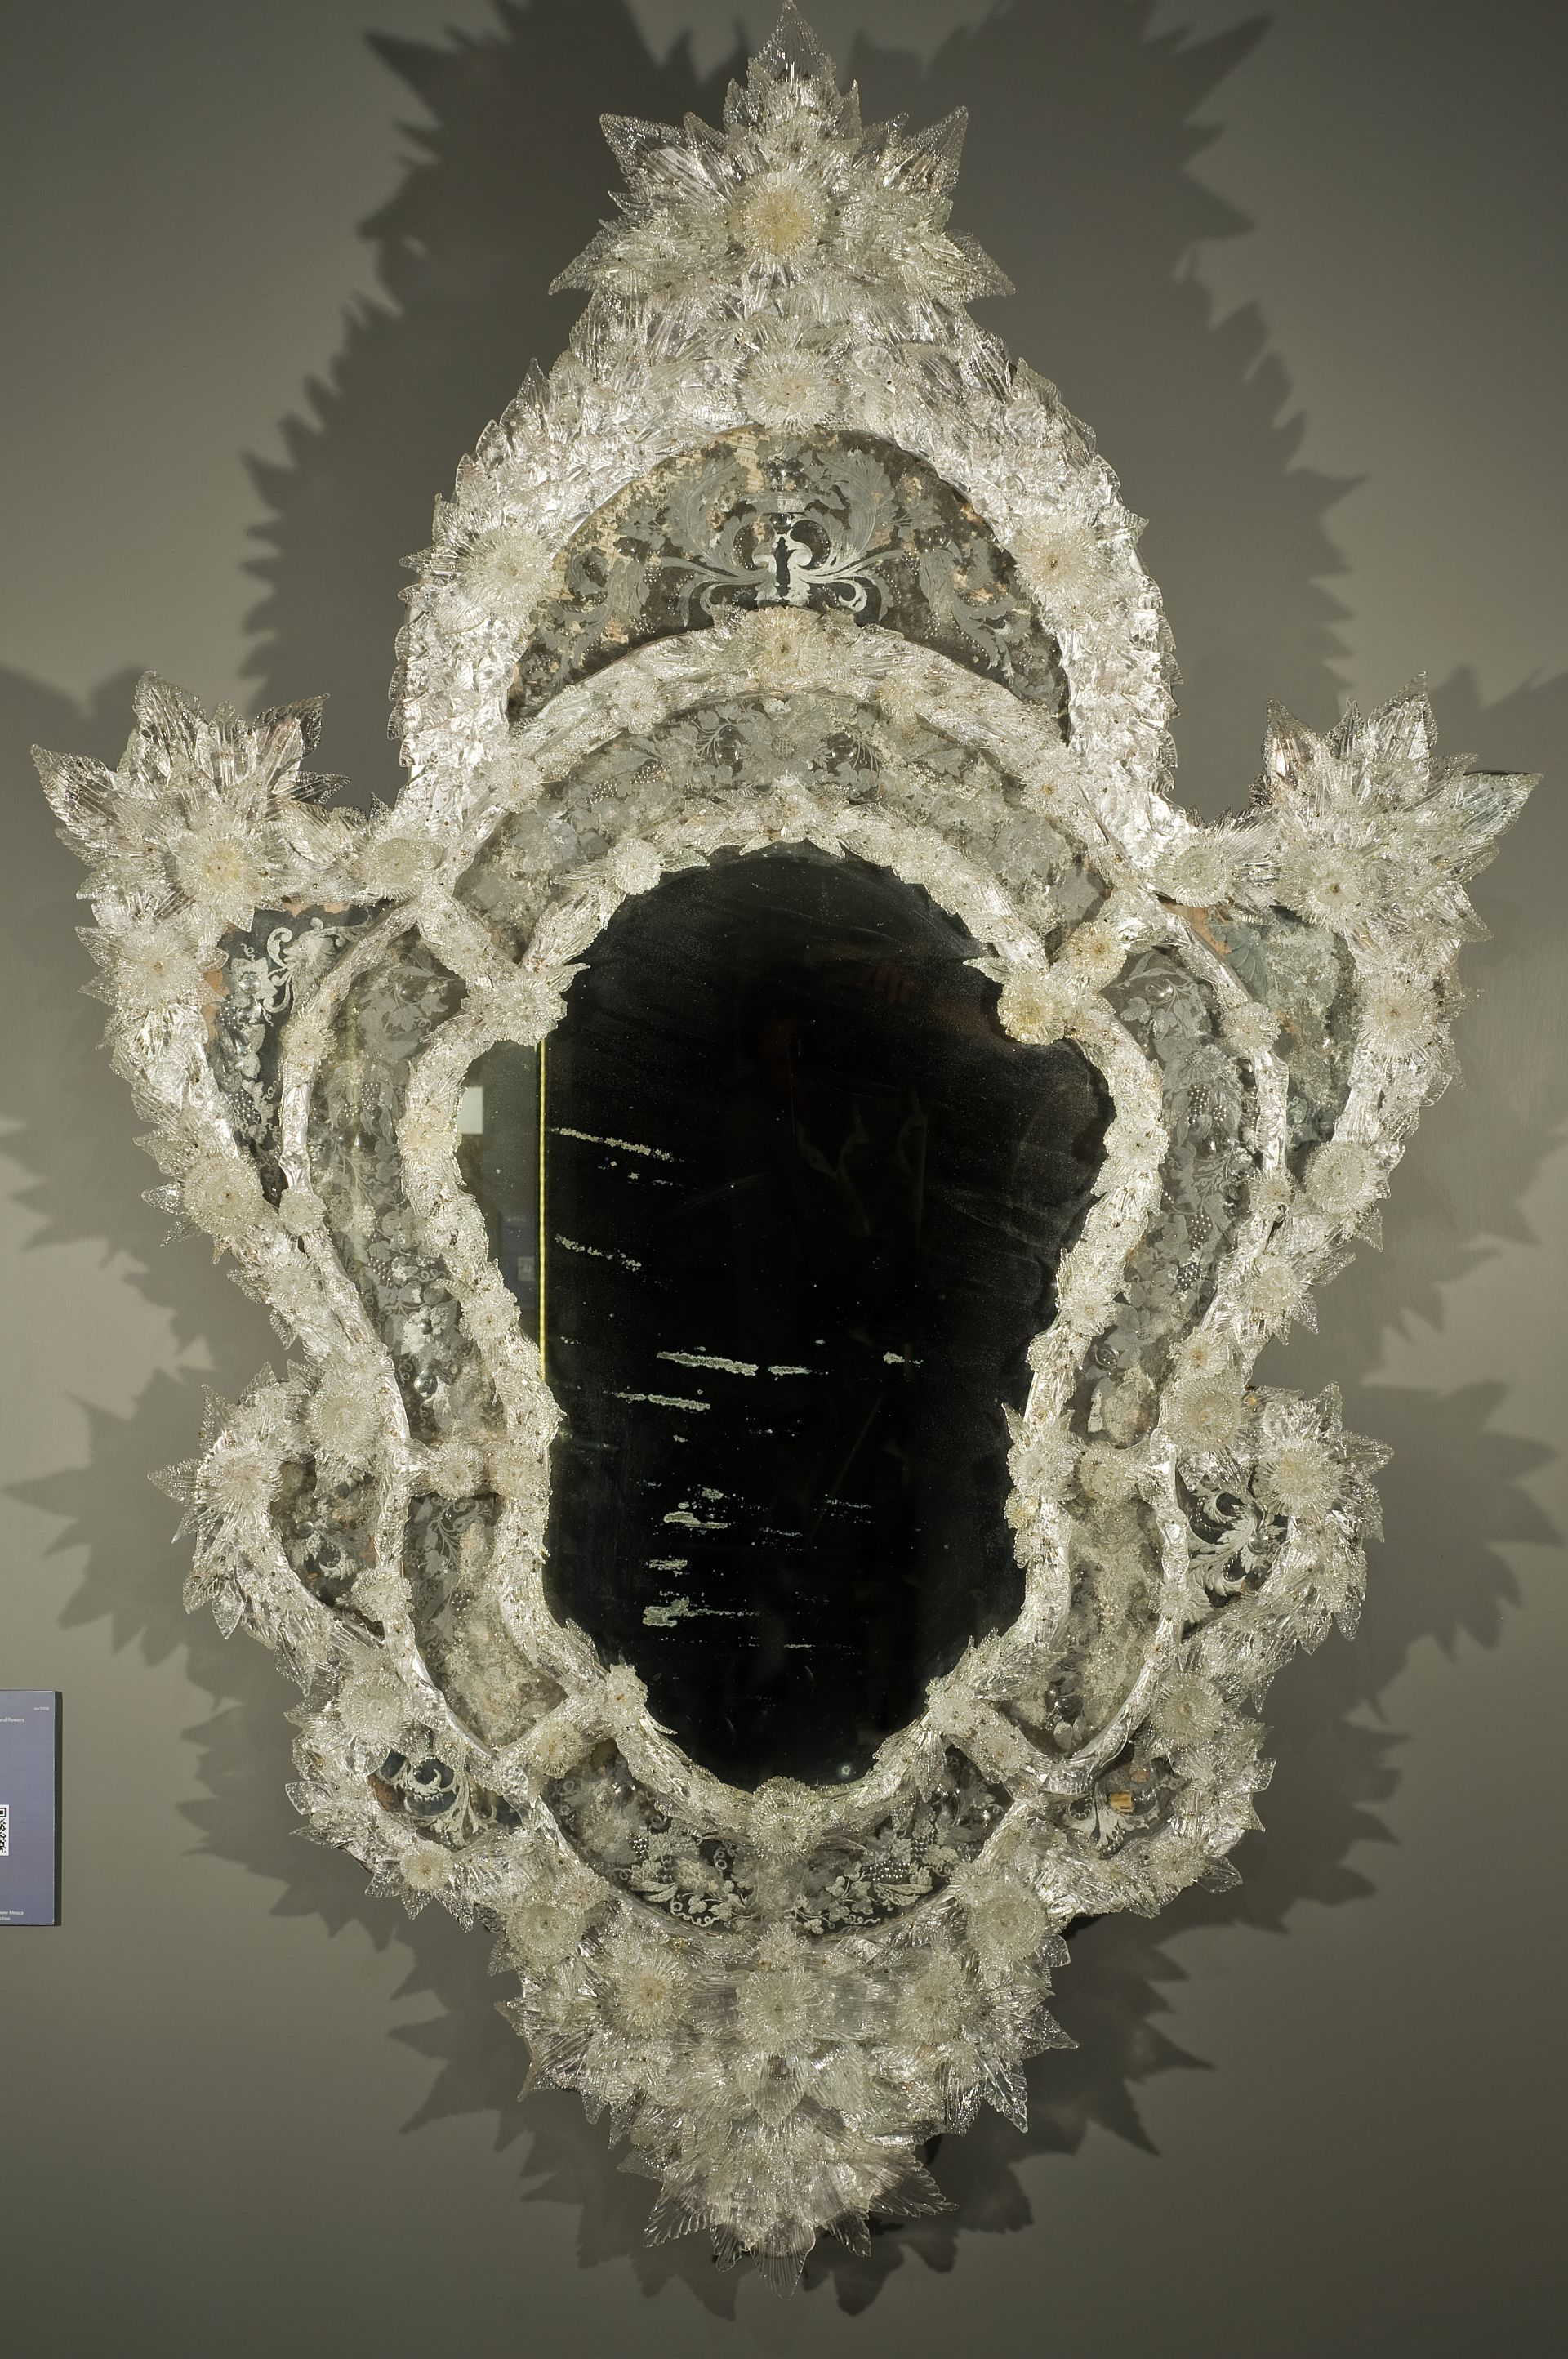
\includegraphics[scale=0.4]{Specchio_di_Murano.jpg}}
			};
		\end{tikzpicture}
	\end{figure}
	
	\begin{minipage}{\linewidth}
		\centering
		\begin{tikzpicture}
			\node[draw,dashed]
			{
				\fboxrule=4pt
				\fcolorbox{white}{white}{
					\fbox{
						\begin{minipage}{80mm}
							\raggedright
							{
								L'opera è una specchiera, si definiscono infatti così gli specchi con cornice creati per essere appesi alle pareti allo scopo di specchiarsi e di decorare le stanze dei nobili tra i quali la Marchesa Toschi Mosca.\\ 
								Realizzata tra la fine del Settecento e l'inizio dell'Ottocento, è decorata con foglie e fiori in vetro e argento che caratterizzano la particolarità delle specchiere artistiche di Murano.
							}
						\end{minipage}
					}
				}
			};
		\end{tikzpicture}
	\end{minipage}
	
	\newpage
	%-------- End image --------
	
	\begin{figure}[h]
		\centering
		\begin{tikzpicture}
			\node[draw,dashed]
			{
				\fboxrule=4pt			
				\fcolorbox{white}{white}{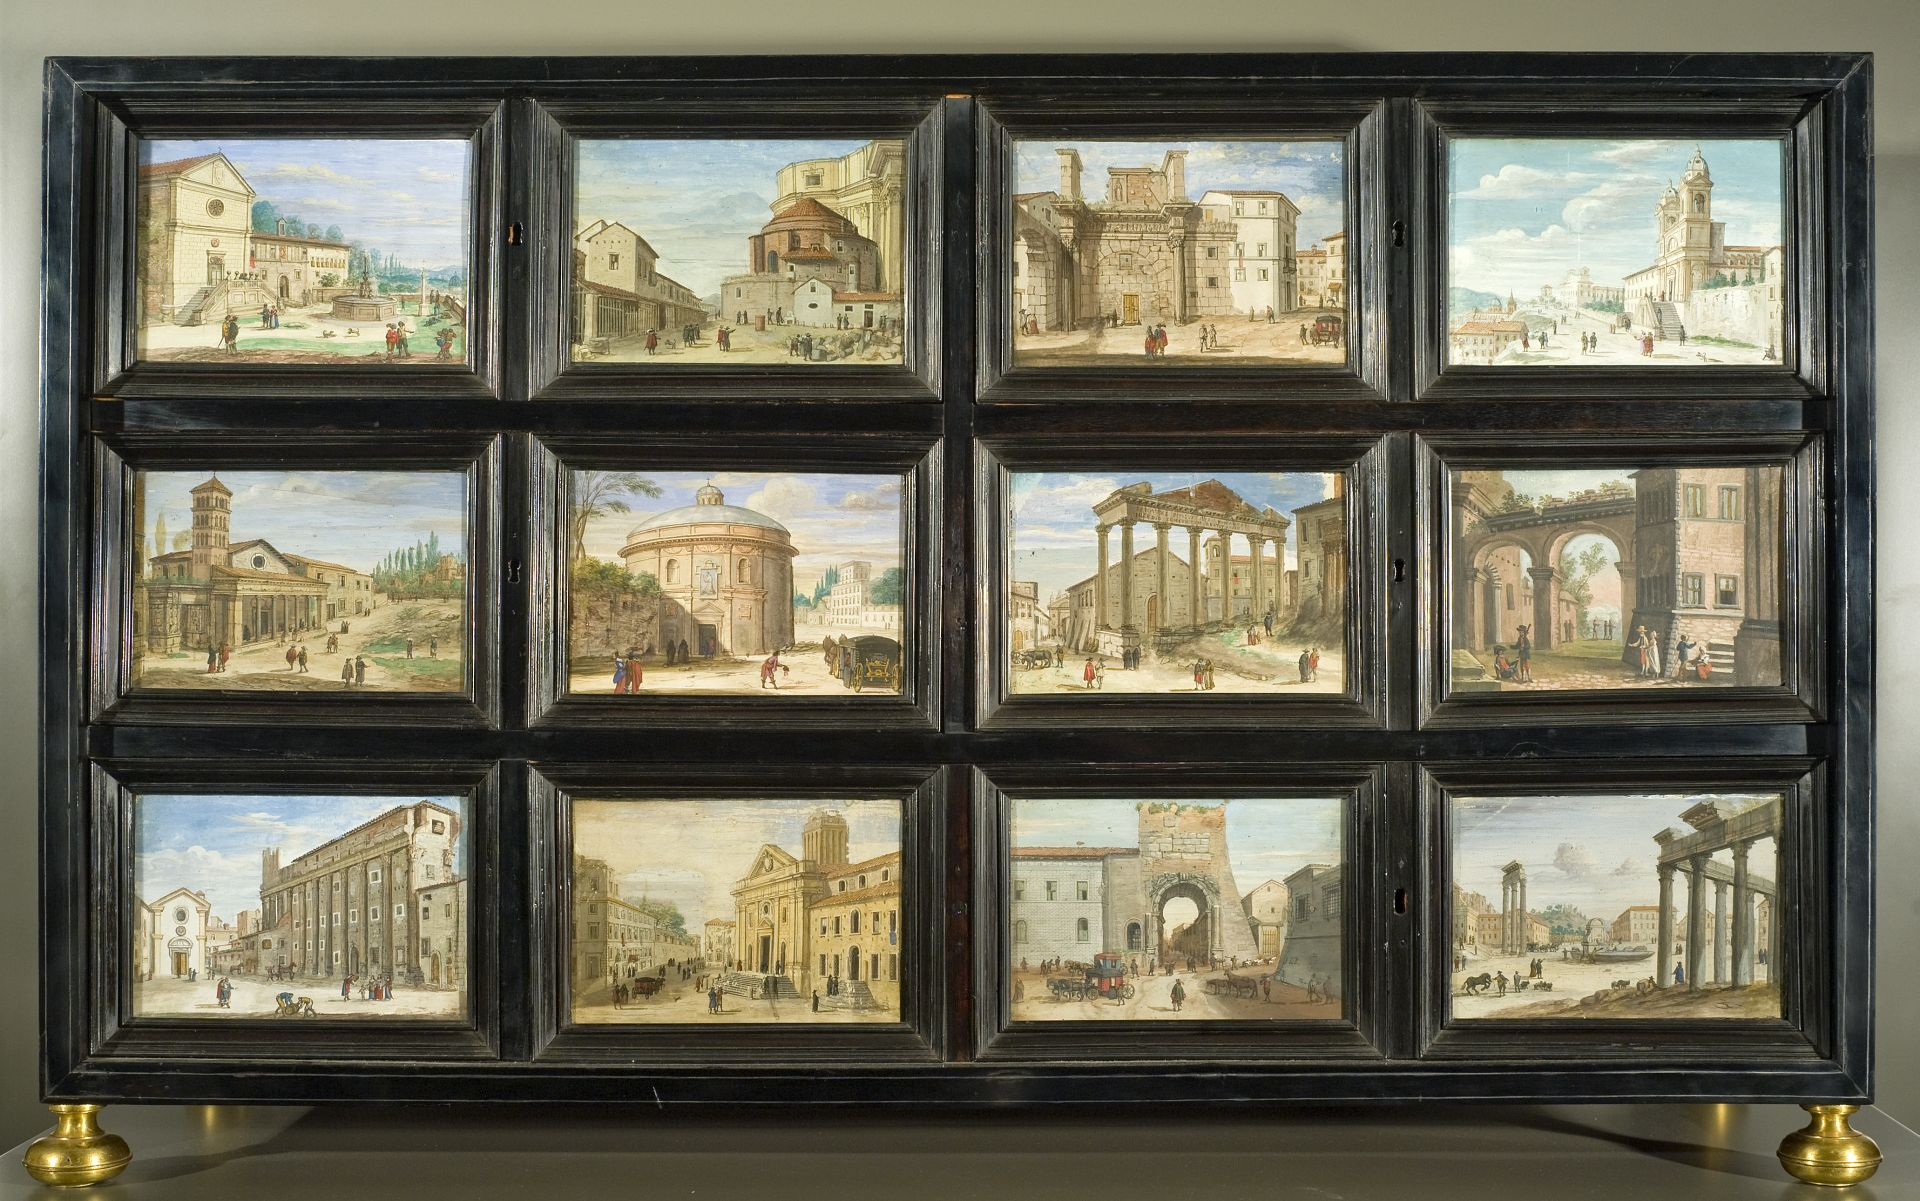
\includegraphics[scale=0.7]{Vedute_di_Roma_1.jpg}}
			};
		\end{tikzpicture}
	\end{figure}
	
	\begin{minipage}{\linewidth}
		\centering
		\begin{tikzpicture}
			\node[draw,dashed]
			{
				\fboxrule=4pt
				\fcolorbox{white}{white}{
					\fbox{
						\begin{minipage}{70mm}
							\raggedright
							{
								Lo Stipo con Vedute di Roma fa parte della Collezione Toschi Mosca, la sua paricolarità è costituita da dei piccoli dipinti realistici del paesaggio romano, realizzati per poter mostrare a mò di cartoline, ai commensali della marchesa i suoi viaggi nella capitale.
							}
						\end{minipage}
					}
				}
			};
		\end{tikzpicture}
	\end{minipage}
	
	\newpage
	%-------- End image --------
	
	\begin{figure}[h]
		\centering
		\begin{tikzpicture}
			\node[draw,dashed]
			{
				\fboxrule=4pt			
				\fcolorbox{white}{white}{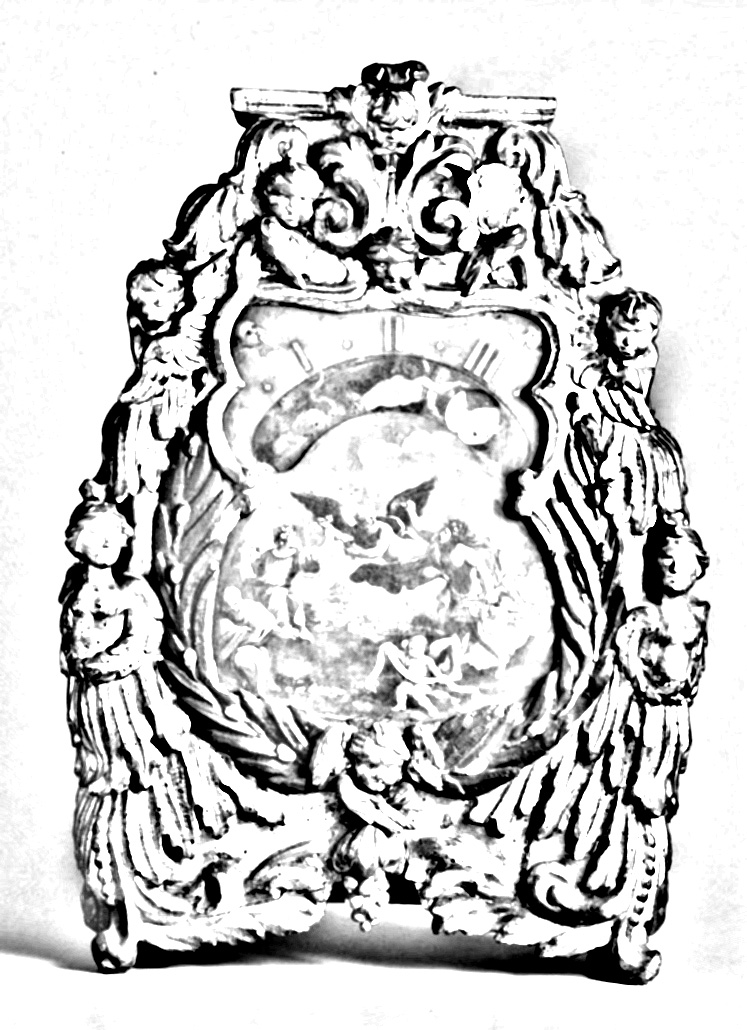
\includegraphics[scale=0.3]{Orologio_notturno.jpg}}
			};
		\end{tikzpicture}
	\end{figure}
	
	\begin{minipage}{\linewidth}
		\centering
		\begin{tikzpicture}
			\node[draw,dashed]
			{
				\fboxrule=4pt
				\fcolorbox{white}{white}{
					\fbox{
						\begin{minipage}{70mm}
							\raggedright
							{
							L'Orologio Notturno è stato realizzato appositamente per la marchesa Toschi Mosca con lo scopo di mostrarle che ore fossero quando si svegliava in preda all'insonnia. L'Orologio è decorato da allegorie che raffigurano lo scorrere inesorabile del tempo.
							}
						\end{minipage}
					}
				}
			};
		\end{tikzpicture}
	\end{minipage}
	
	\newpage
	%-------- End image --------
	
	\begin{figure}[h]
		\centering
		\begin{tikzpicture}
			\node[draw,dashed]
			{
				\fboxrule=4pt			
				\fcolorbox{white}{white}{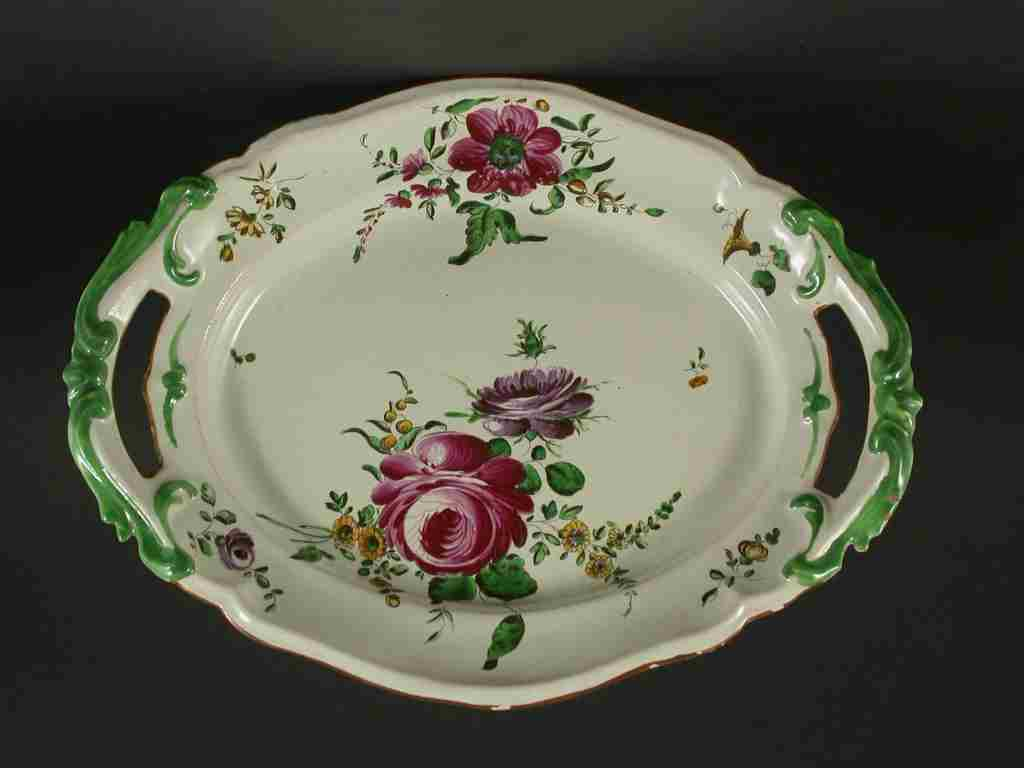
\includegraphics[scale=1.2]{Scacciani_Antonio-Vassoio-Rosa.jpg}}
			};
		\end{tikzpicture}
	\end{figure}
	
	\begin{minipage}{\linewidth}
		\centering
		\begin{tikzpicture}
			\node[draw,dashed]
			{
				\fboxrule=4pt
				\fcolorbox{white}{white}{
					\fbox{
						\begin{minipage}{60mm}
							\raggedright
							{
								 Il Grande piatto è munito di due manici dipinti in color verde smeraldo ed è decorato con il tipico motivo "alla rosa di Pesaro" caratteristico della nostra zona. 
							}
						\end{minipage}
					}
				}
			};
		\end{tikzpicture}
	\end{minipage}
	
	\newpage
	%-------- End image --------
	
	\begin{figure}[h]
		\centering
		\begin{tikzpicture}
			\node[draw,dashed]
			{
				\fboxrule=4pt			
				\fcolorbox{white}{white}{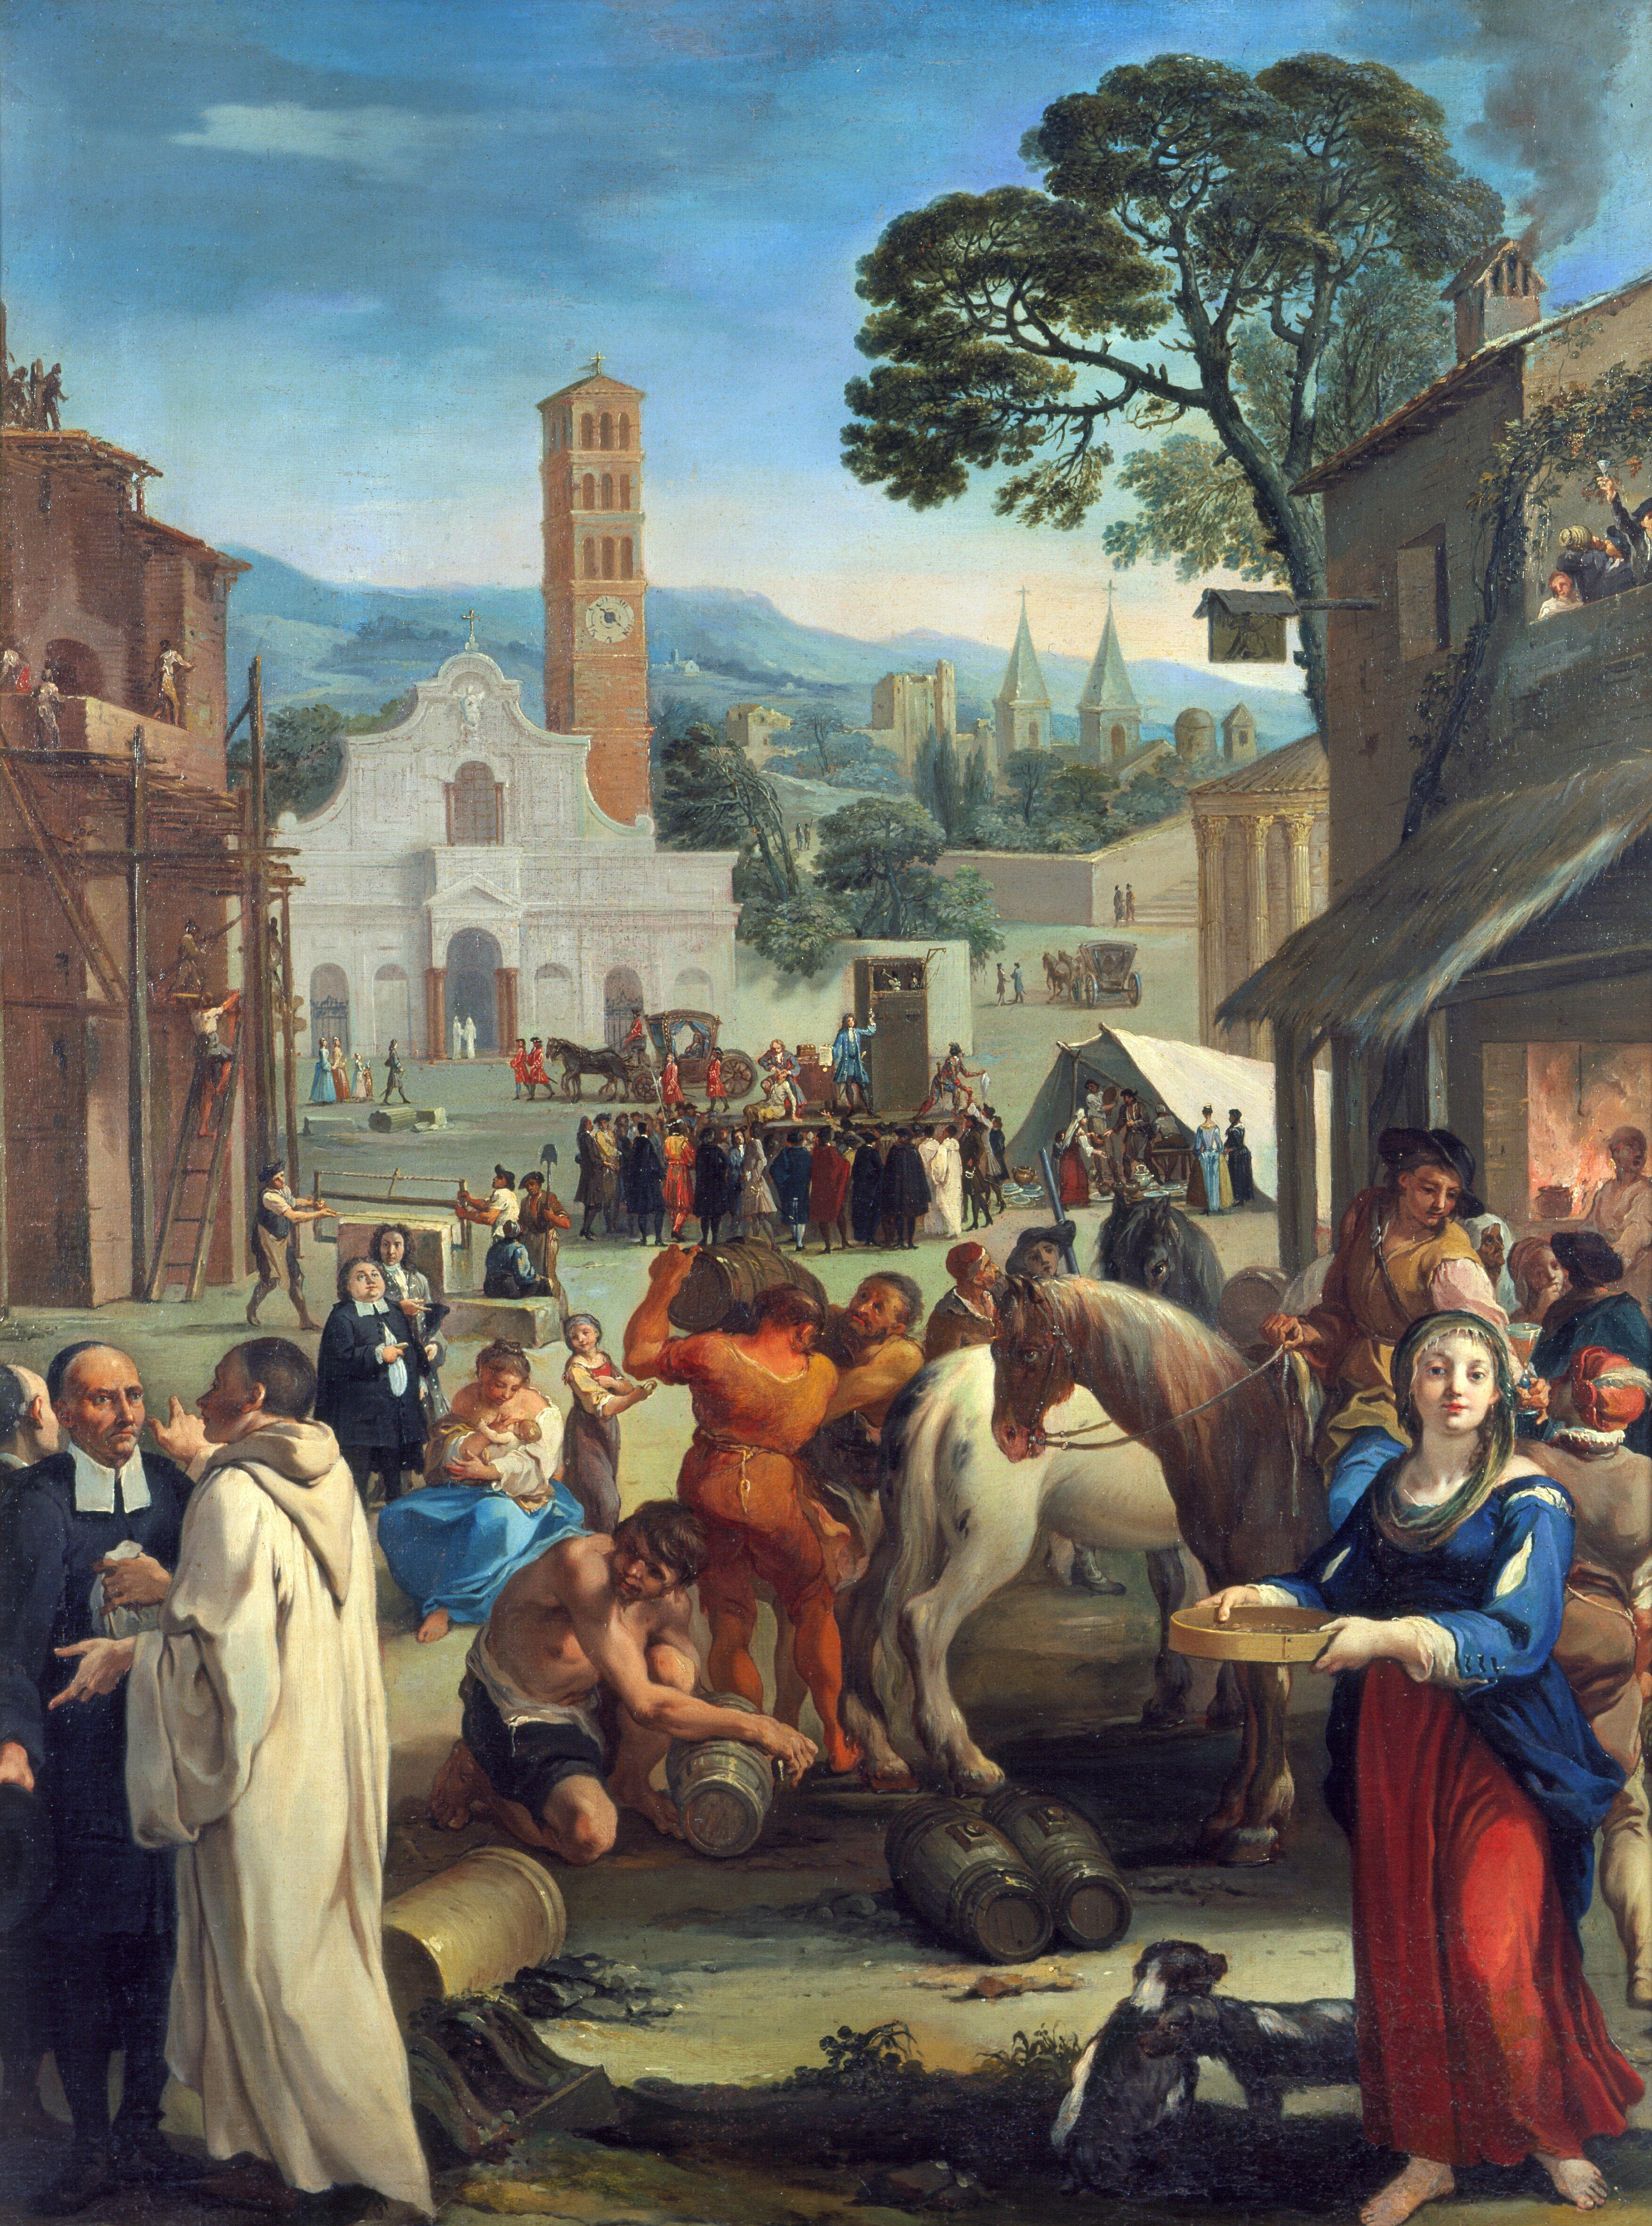
\includegraphics[scale=0.068]{Milani_Aureliano-Mercato.jpg}}
			};
		\end{tikzpicture}
	\end{figure}
	
	\begin{minipage}{\linewidth}
		\centering
		\begin{tikzpicture}
			\node[draw,dashed]
			{
				\fboxrule=4pt
				\fcolorbox{white}{white}{
					\fbox{
						\begin{minipage}{90mm}
							\raggedright
							{
								Il dipinto raffigura una piazza circondata da costruzioni moderne e più antiche ed un alto albero, è attorniata da ruderi sparsi a terra. In essa si trovano alcune scene popolari come:"una donna con setaccio in primo piano e tre religiosi sul lato opposto". Al centro sono rappresentati alcuni uomini che sollevano barili; vi è un gruppo di curiosi davanti ad un teatrino, e, dietro, è raffigurata una carrozzina trainata da cavalli, che attraversa lo spazio davanti alla facciata di una chiesa. In questo dipinto sono quindi distinguibili nella loro quotidianità esponenti di diversi ceti sociali e i relativi mestieri.
							}
						\end{minipage}
					}
				}
			};
		\end{tikzpicture}
	\end{minipage}
	
	\newpage
	%-------- End image --------
	
	\begin{figure}[h]
		\centering
		\begin{tikzpicture}
			\node[draw,dashed]
			{
				\fboxrule=4pt			
				\fcolorbox{white}{white}{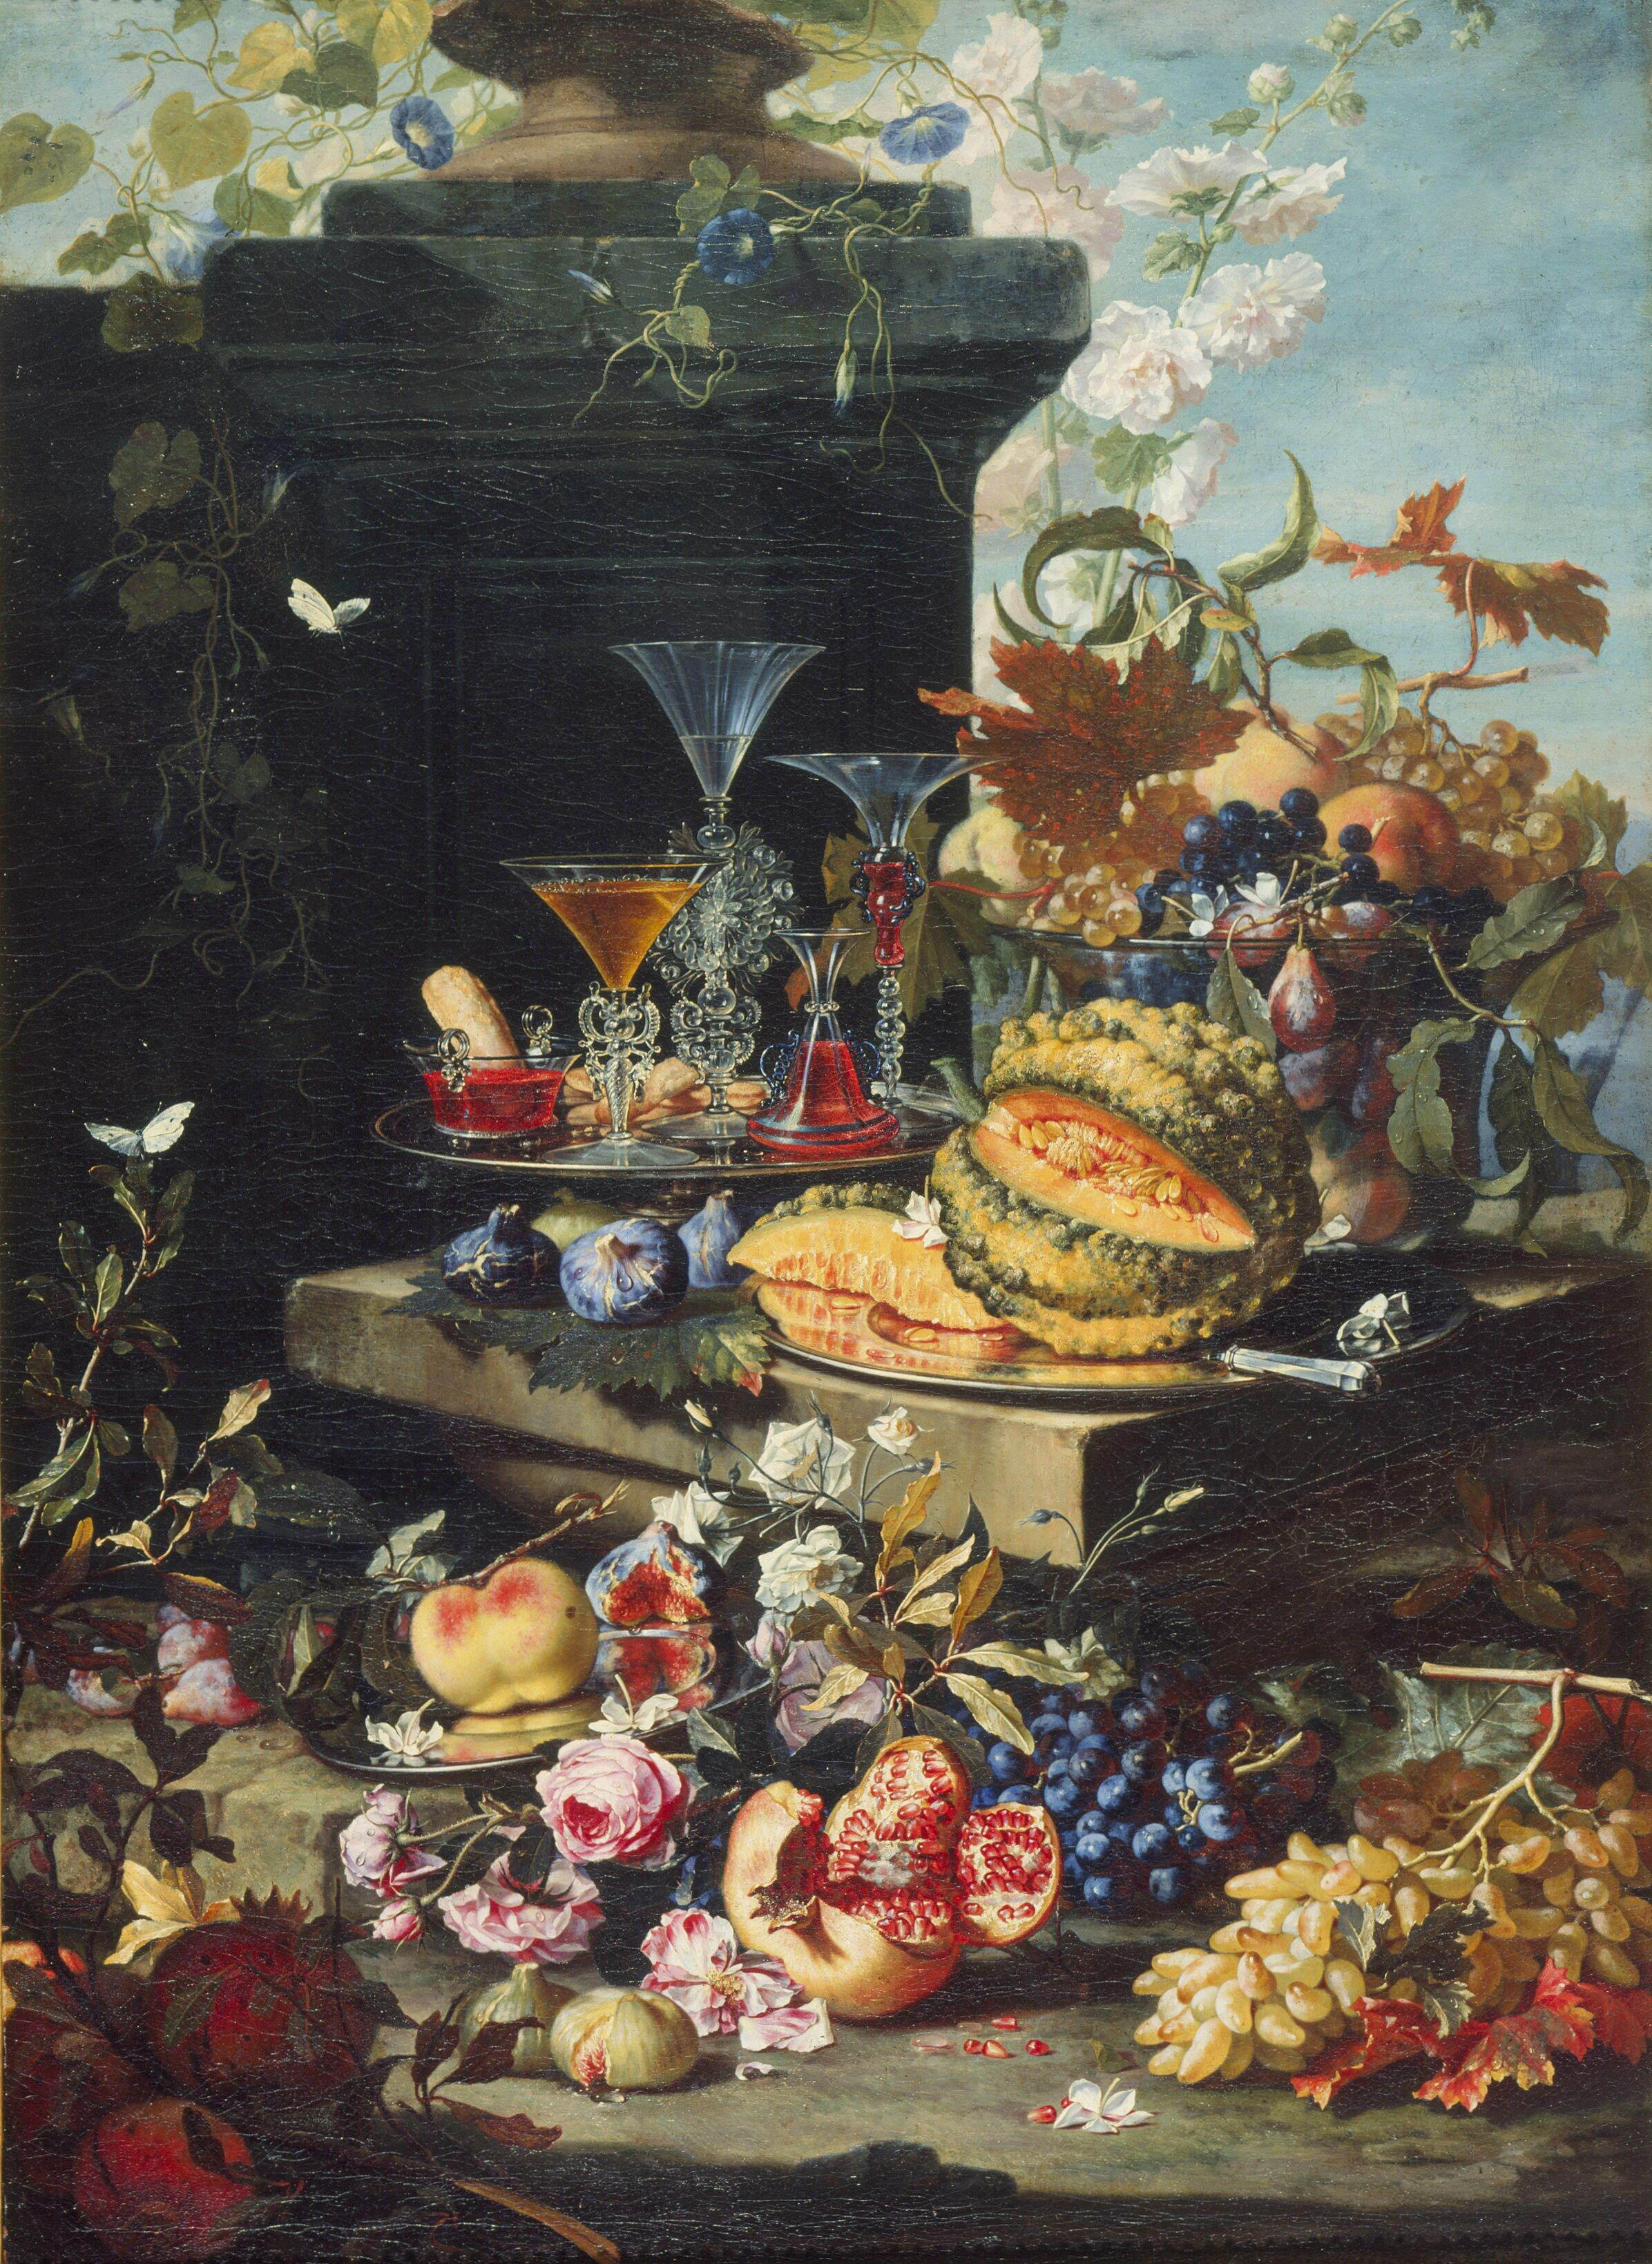
\includegraphics[scale= 0.1]{Berentz_Christian-Fiori_e_frutta_con_bicchieri_di_cristallo.jpg}}
			};
		\end{tikzpicture}
	\end{figure}
	
	\begin{minipage}{\linewidth}
		\centering
		\begin{tikzpicture}
			\node[draw,dashed]
			{
				\fboxrule=4pt
				\fcolorbox{white}{white}{
					\fbox{
						\begin{minipage}{90mm}
							\raggedright
							{
								ll dipinto raffigura diverse frutta, fiori e ramoscelli disposti su diversi piani formati da rocce, una lastra di pietra, un muretto con colonna in alto. In particolare in primo piano si vede una grossa melagrana aperta, un grappolo d' uva  e sopra una zucca con una fetta mancante; dietro vi è un'alzata che sorregge alcuni bicchieri. Due farfalle voleggiano a sinistra per raggiungere i fiori a decorazione del muretto. L'abbondanza della frutta e dei liquori è accompagnata dall'effimera precarietà della loro freschezza, metafora della breve durata della giovinezza.
							}
						\end{minipage}
					}
				}
			};
		\end{tikzpicture}
	\end{minipage}
	
	\newpage
	%-------- End image --------
	
	\begin{figure}[h]
		\centering
		\begin{tikzpicture}
			\node[draw,dashed]
			{
				\fboxrule=4pt			
				\fcolorbox{white}{white}{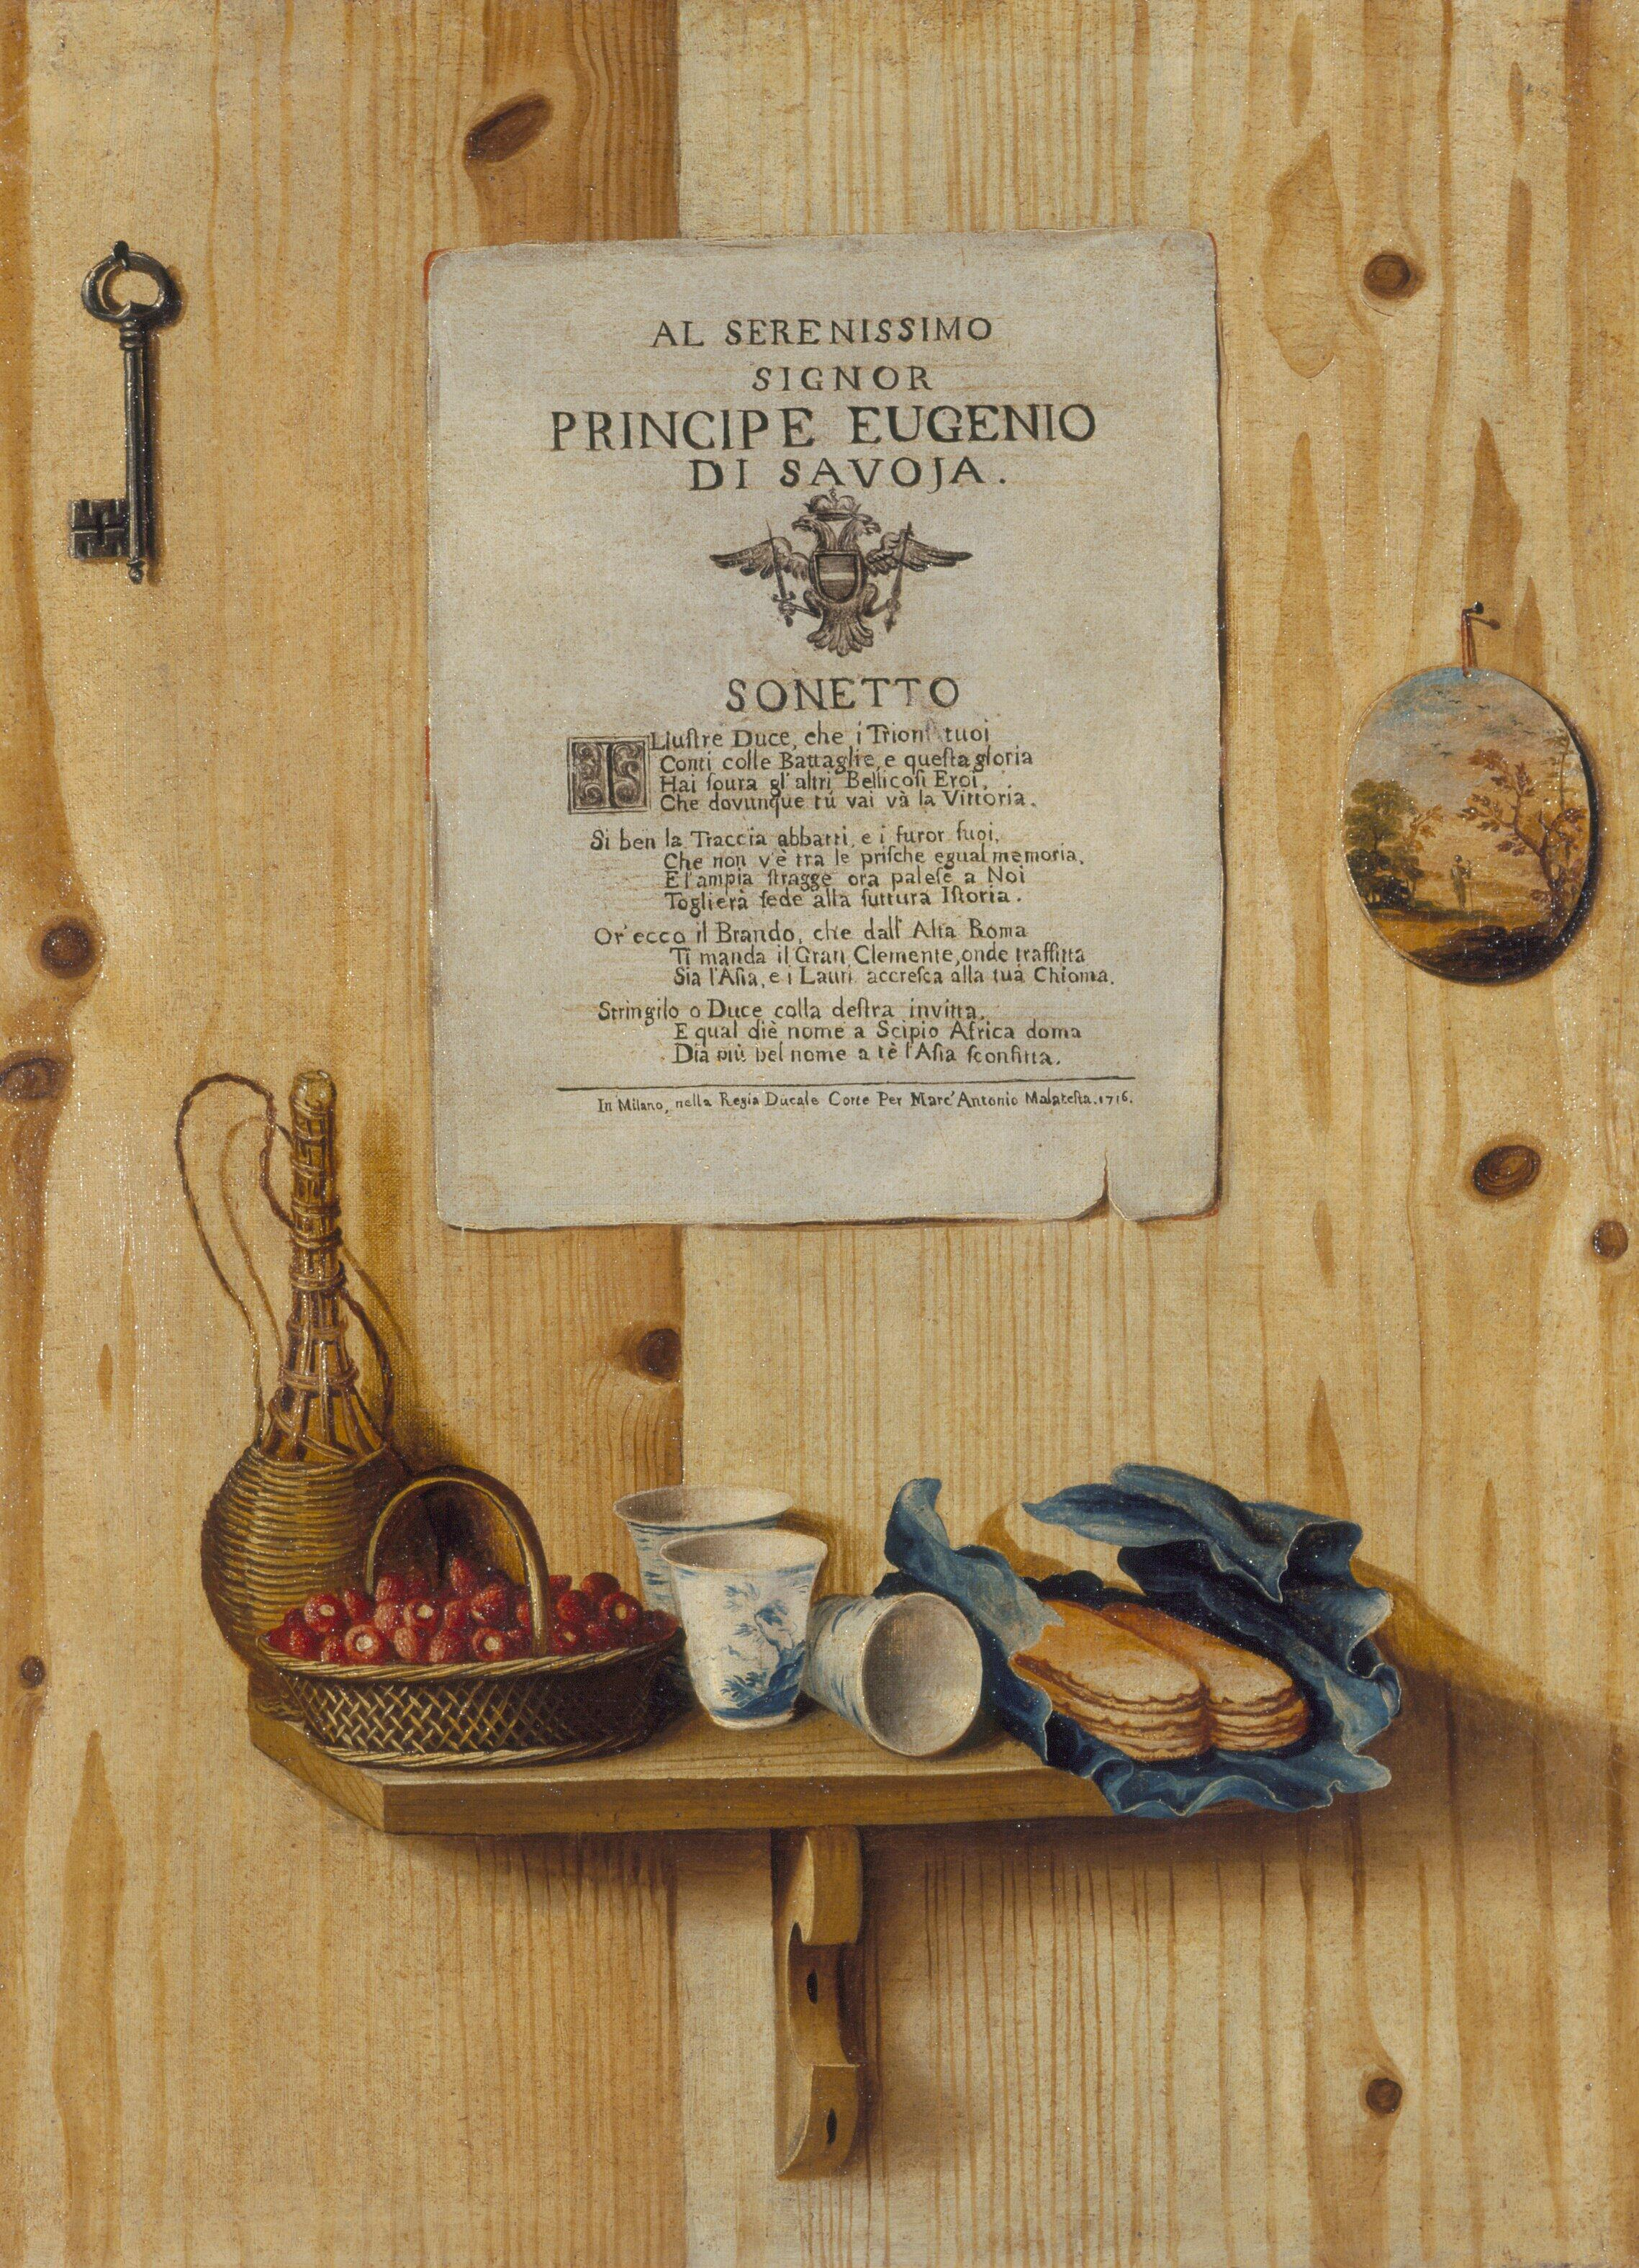
\includegraphics[scale=0.12]{Gianlisi_Antonio_Junior-Trompe_l_oeil_con_sonetto_in_onore_di_Eugenio_di_Savoia_e_mensola_con_oggetti.jpg}}
			};
		\end{tikzpicture}
	\end{figure}
	
	\begin{minipage}{\linewidth}
		\centering
		\begin{tikzpicture}
			\node[draw,dashed]
			{
				\fboxrule=4pt
				\fcolorbox{white}{white}{
					\fbox{
						\begin{minipage}{60mm}
							\raggedright
							{
							Il Trompe l'oeil con sonetto in onore di Eugenio di Savoia. Il Tromple l'oeil è abbellito da una mensola con sopra collocati oggetti di uso comune, tra i quali tazzine, cestino di more, una fiasca di vino e il dettaglio dei biscotti Savoiardi che richiamano la stirpe dei Savoia.
							}
						\end{minipage}
					}
				}
			};
		\end{tikzpicture}
	\end{minipage}
	
	\newpage
	%-------- End image --------
	
	\begin{figure}[h]
		\centering
		\begin{tikzpicture}
			\node[draw,dashed]
			{
				\fboxrule=4pt			
				\fcolorbox{white}{white}{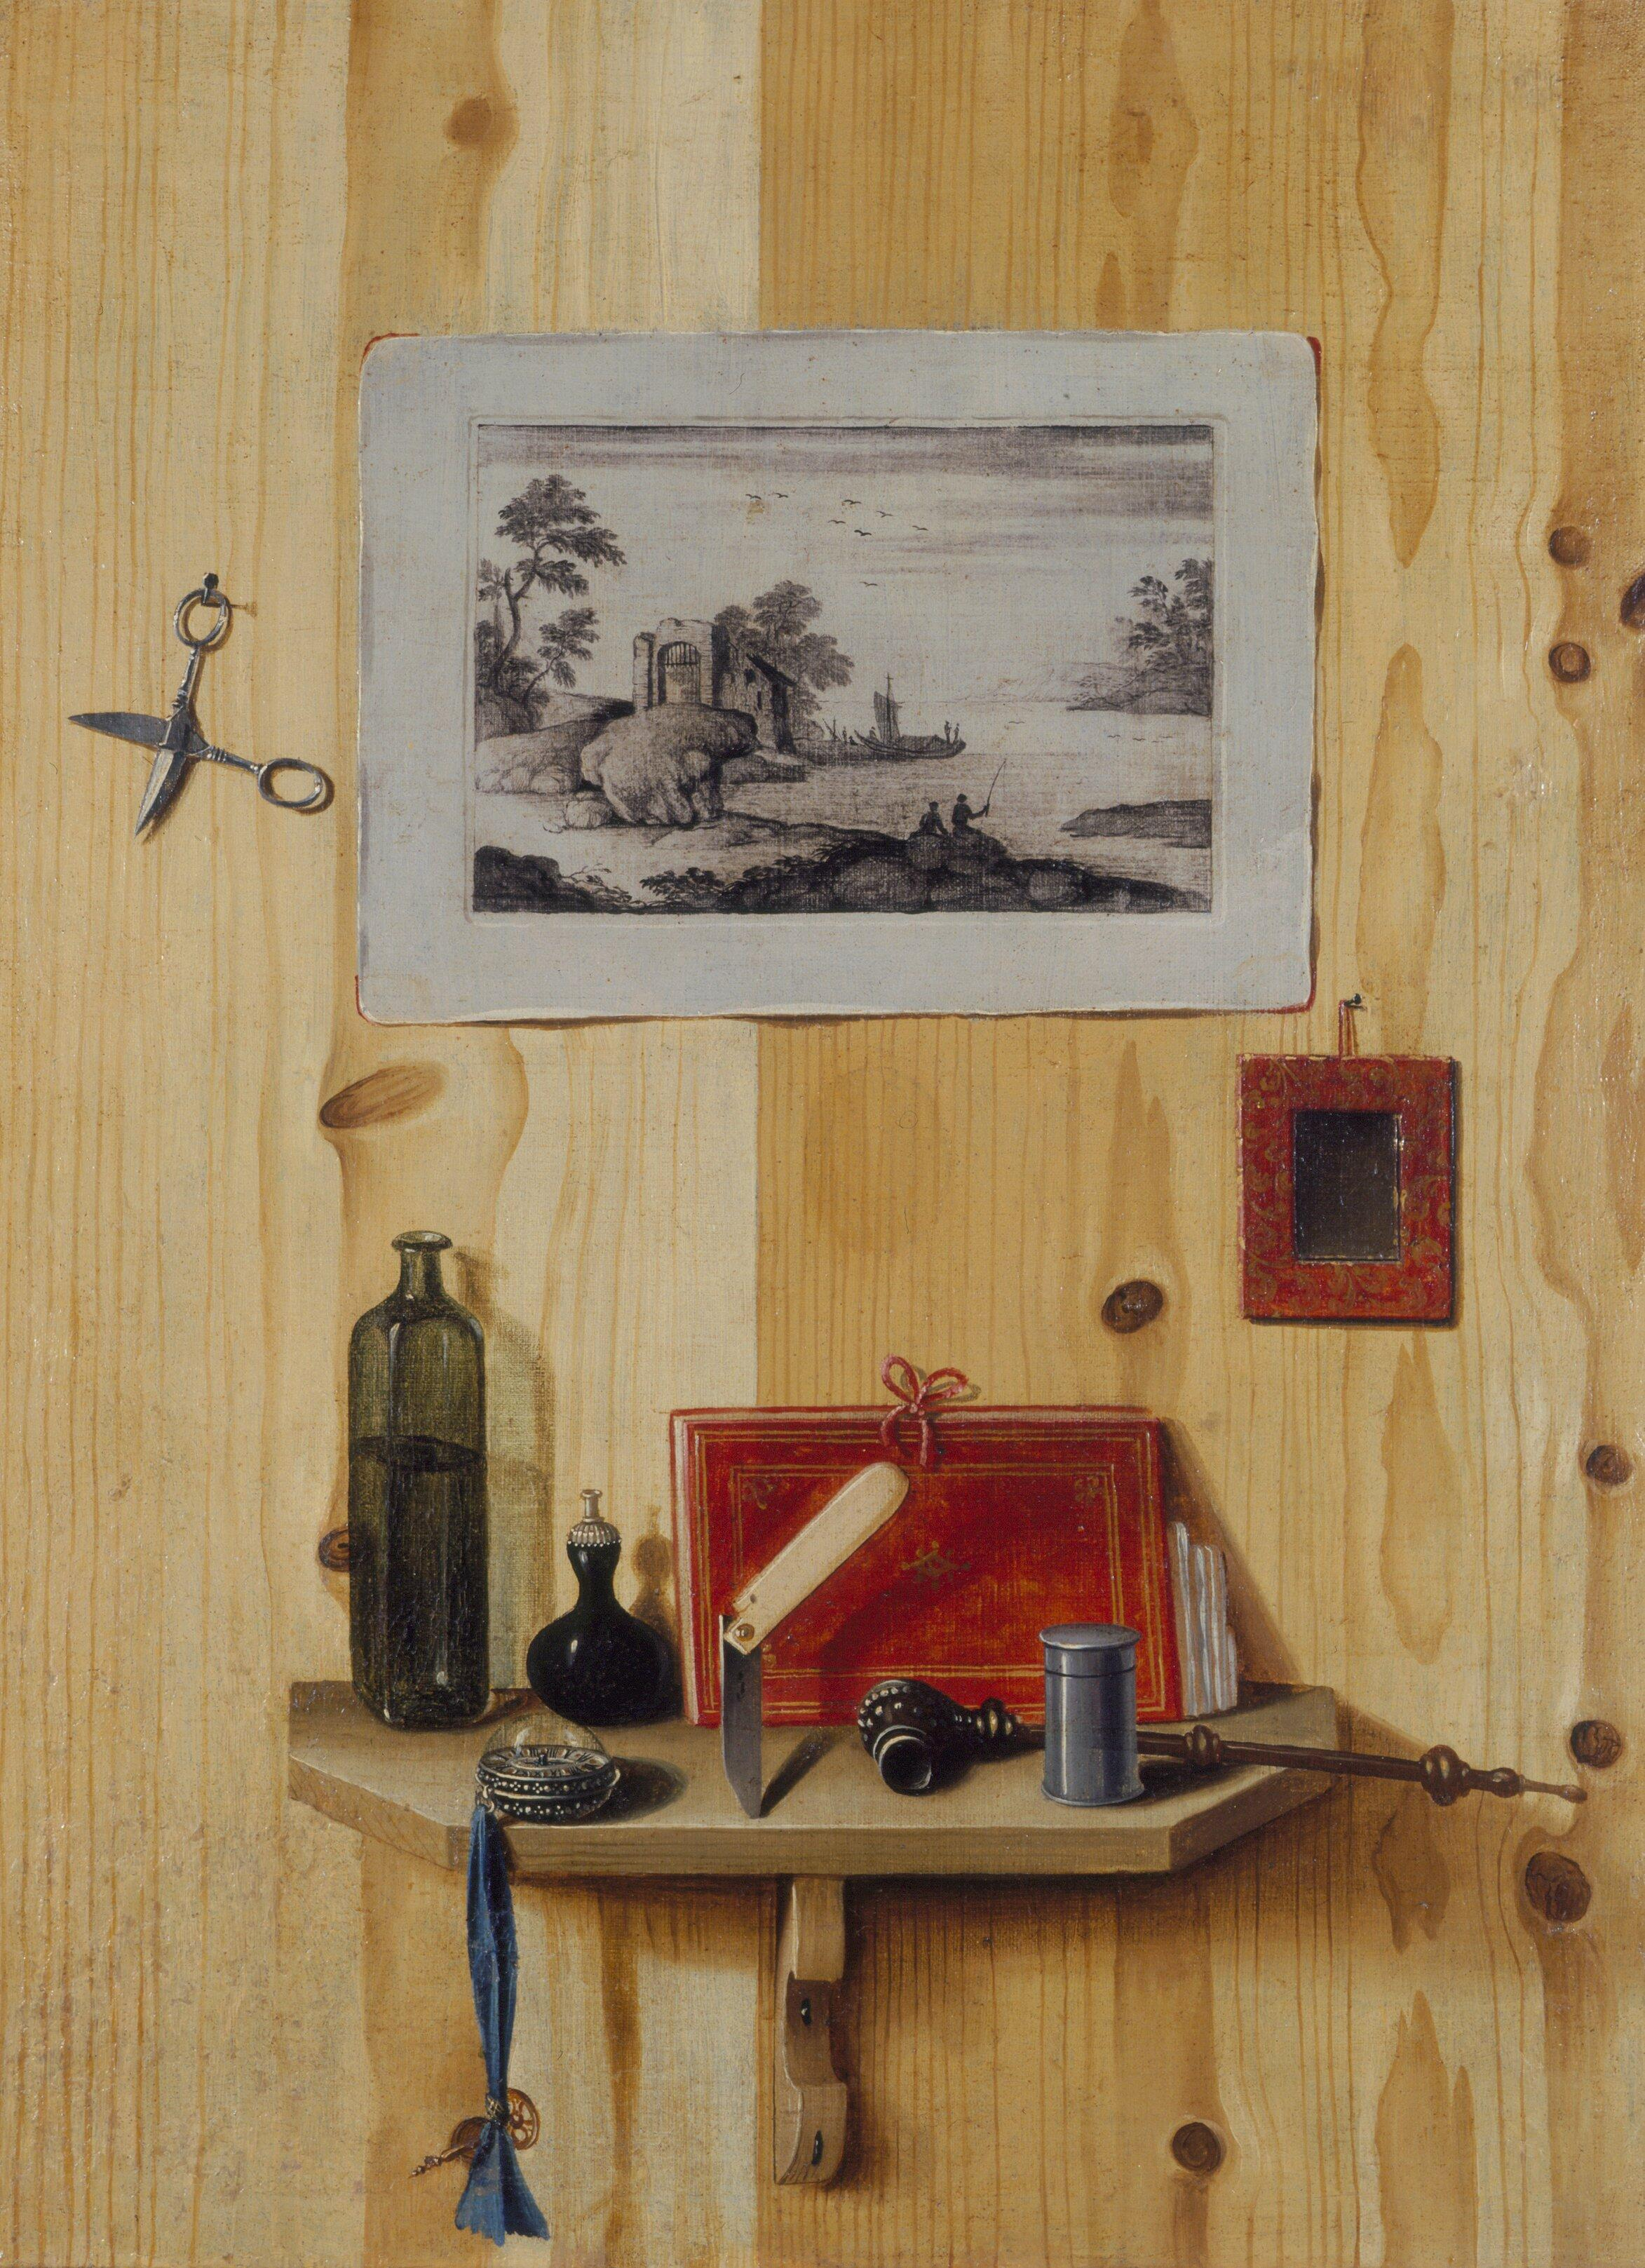
\includegraphics[scale=0.12]{Gianlisi_Antonio_Junior-Trompe_l_oeil_con_paesaggio_forbici_e_mensola_con_oggetti.jpg}}
			};
		\end{tikzpicture}
	\end{figure}
	
	\begin{minipage}{\linewidth}
		\centering
		\begin{tikzpicture}
			\node[draw,dashed]
			{
				\fboxrule=4pt
				\fcolorbox{white}{white}{
					\fbox{
						\begin{minipage}{90mm}
							\raggedright
							{
								Il Tromple l'oeil è fatto in maniera da sembrare una parete di legno, sulla quale sono appese con un chiodo delle forbici, ed è stata fissata una stampa con paesaggio ed un quadretto, più in basso è posto un ripiano con sopra una bottiglia, un calamaio, un libro, una pipa, un coltello a serramanico e una medaglia. 
							}
						\end{minipage}
					}
				}
			};
		\end{tikzpicture}
	\end{minipage}
	
	\newpage
	%-------- End image --------
	
	\begin{figure}[h]
		\centering
		\begin{tikzpicture}
			\node[draw,dashed]
			{
				\fboxrule=4pt			
				\fcolorbox{white}{white}{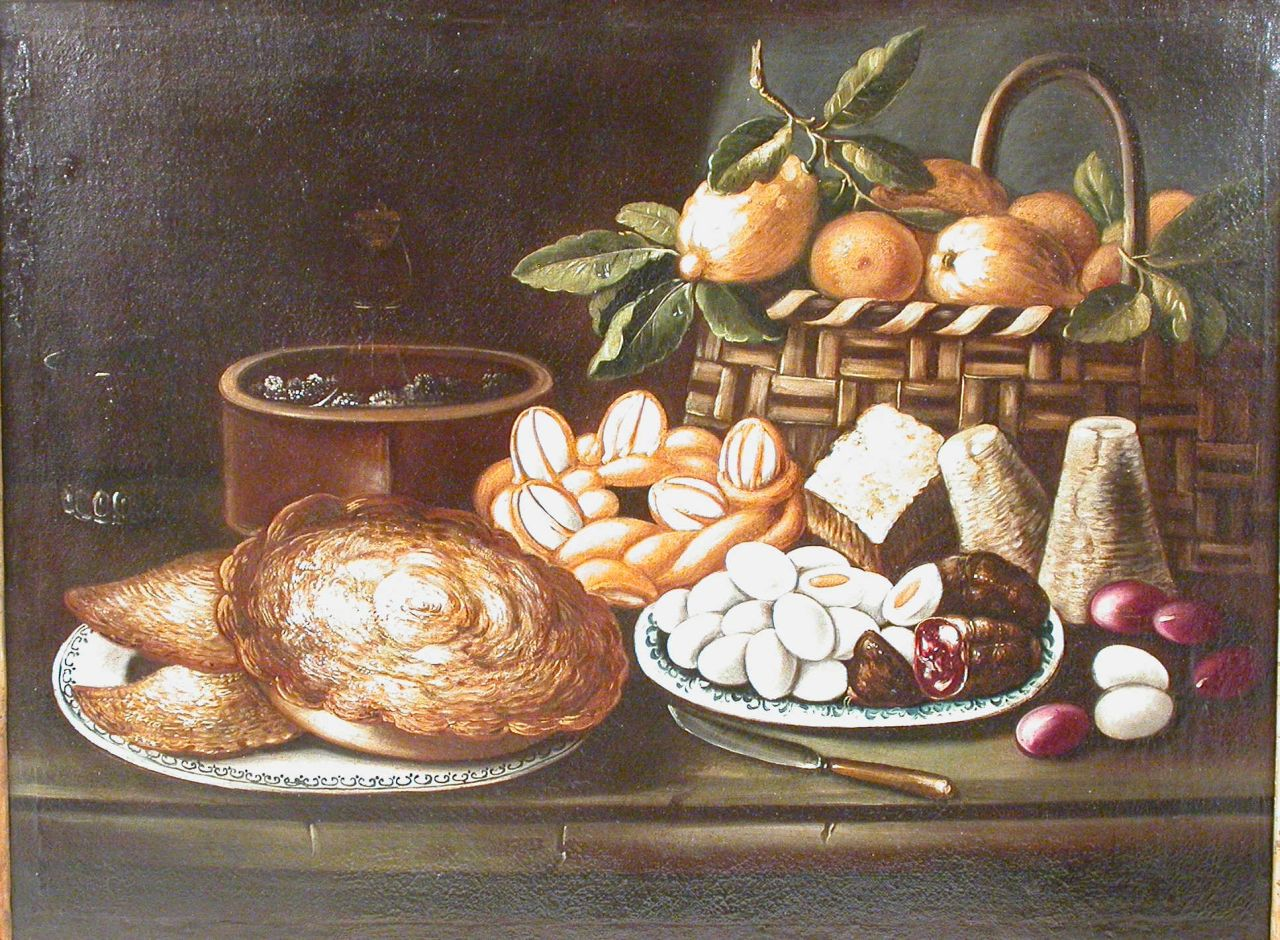
\includegraphics[scale=1.2]{Realfonzo_Tommaso-Natura_morta_con_dolci_frutta_uova_e_formaggi.jpg}}
			};
		\end{tikzpicture}
	\end{figure}
	
	\begin{minipage}{\linewidth}
		\centering
		\begin{tikzpicture}
			\node[draw,dashed]
			{
				\fboxrule=4pt
				\fcolorbox{white}{white}{
					\fbox{
						\begin{minipage}{60mm}
							\raggedright
							{
								Il dipinto raffigura  una natura morta con dolci, uova, formaggi, salami, uova e un cesto di limoni. Il banchetto è probabilmente simbolo della festa Pasquale.
							}
						\end{minipage}
					}
				}
			};
		\end{tikzpicture}
	\end{minipage}
	
	\newpage
	%-------- End image --------
	
	\begin{figure}[h]
		\centering
		\begin{tikzpicture}
			\node[draw,dashed]
			{
				\fboxrule=4pt			
				\fcolorbox{white}{white}{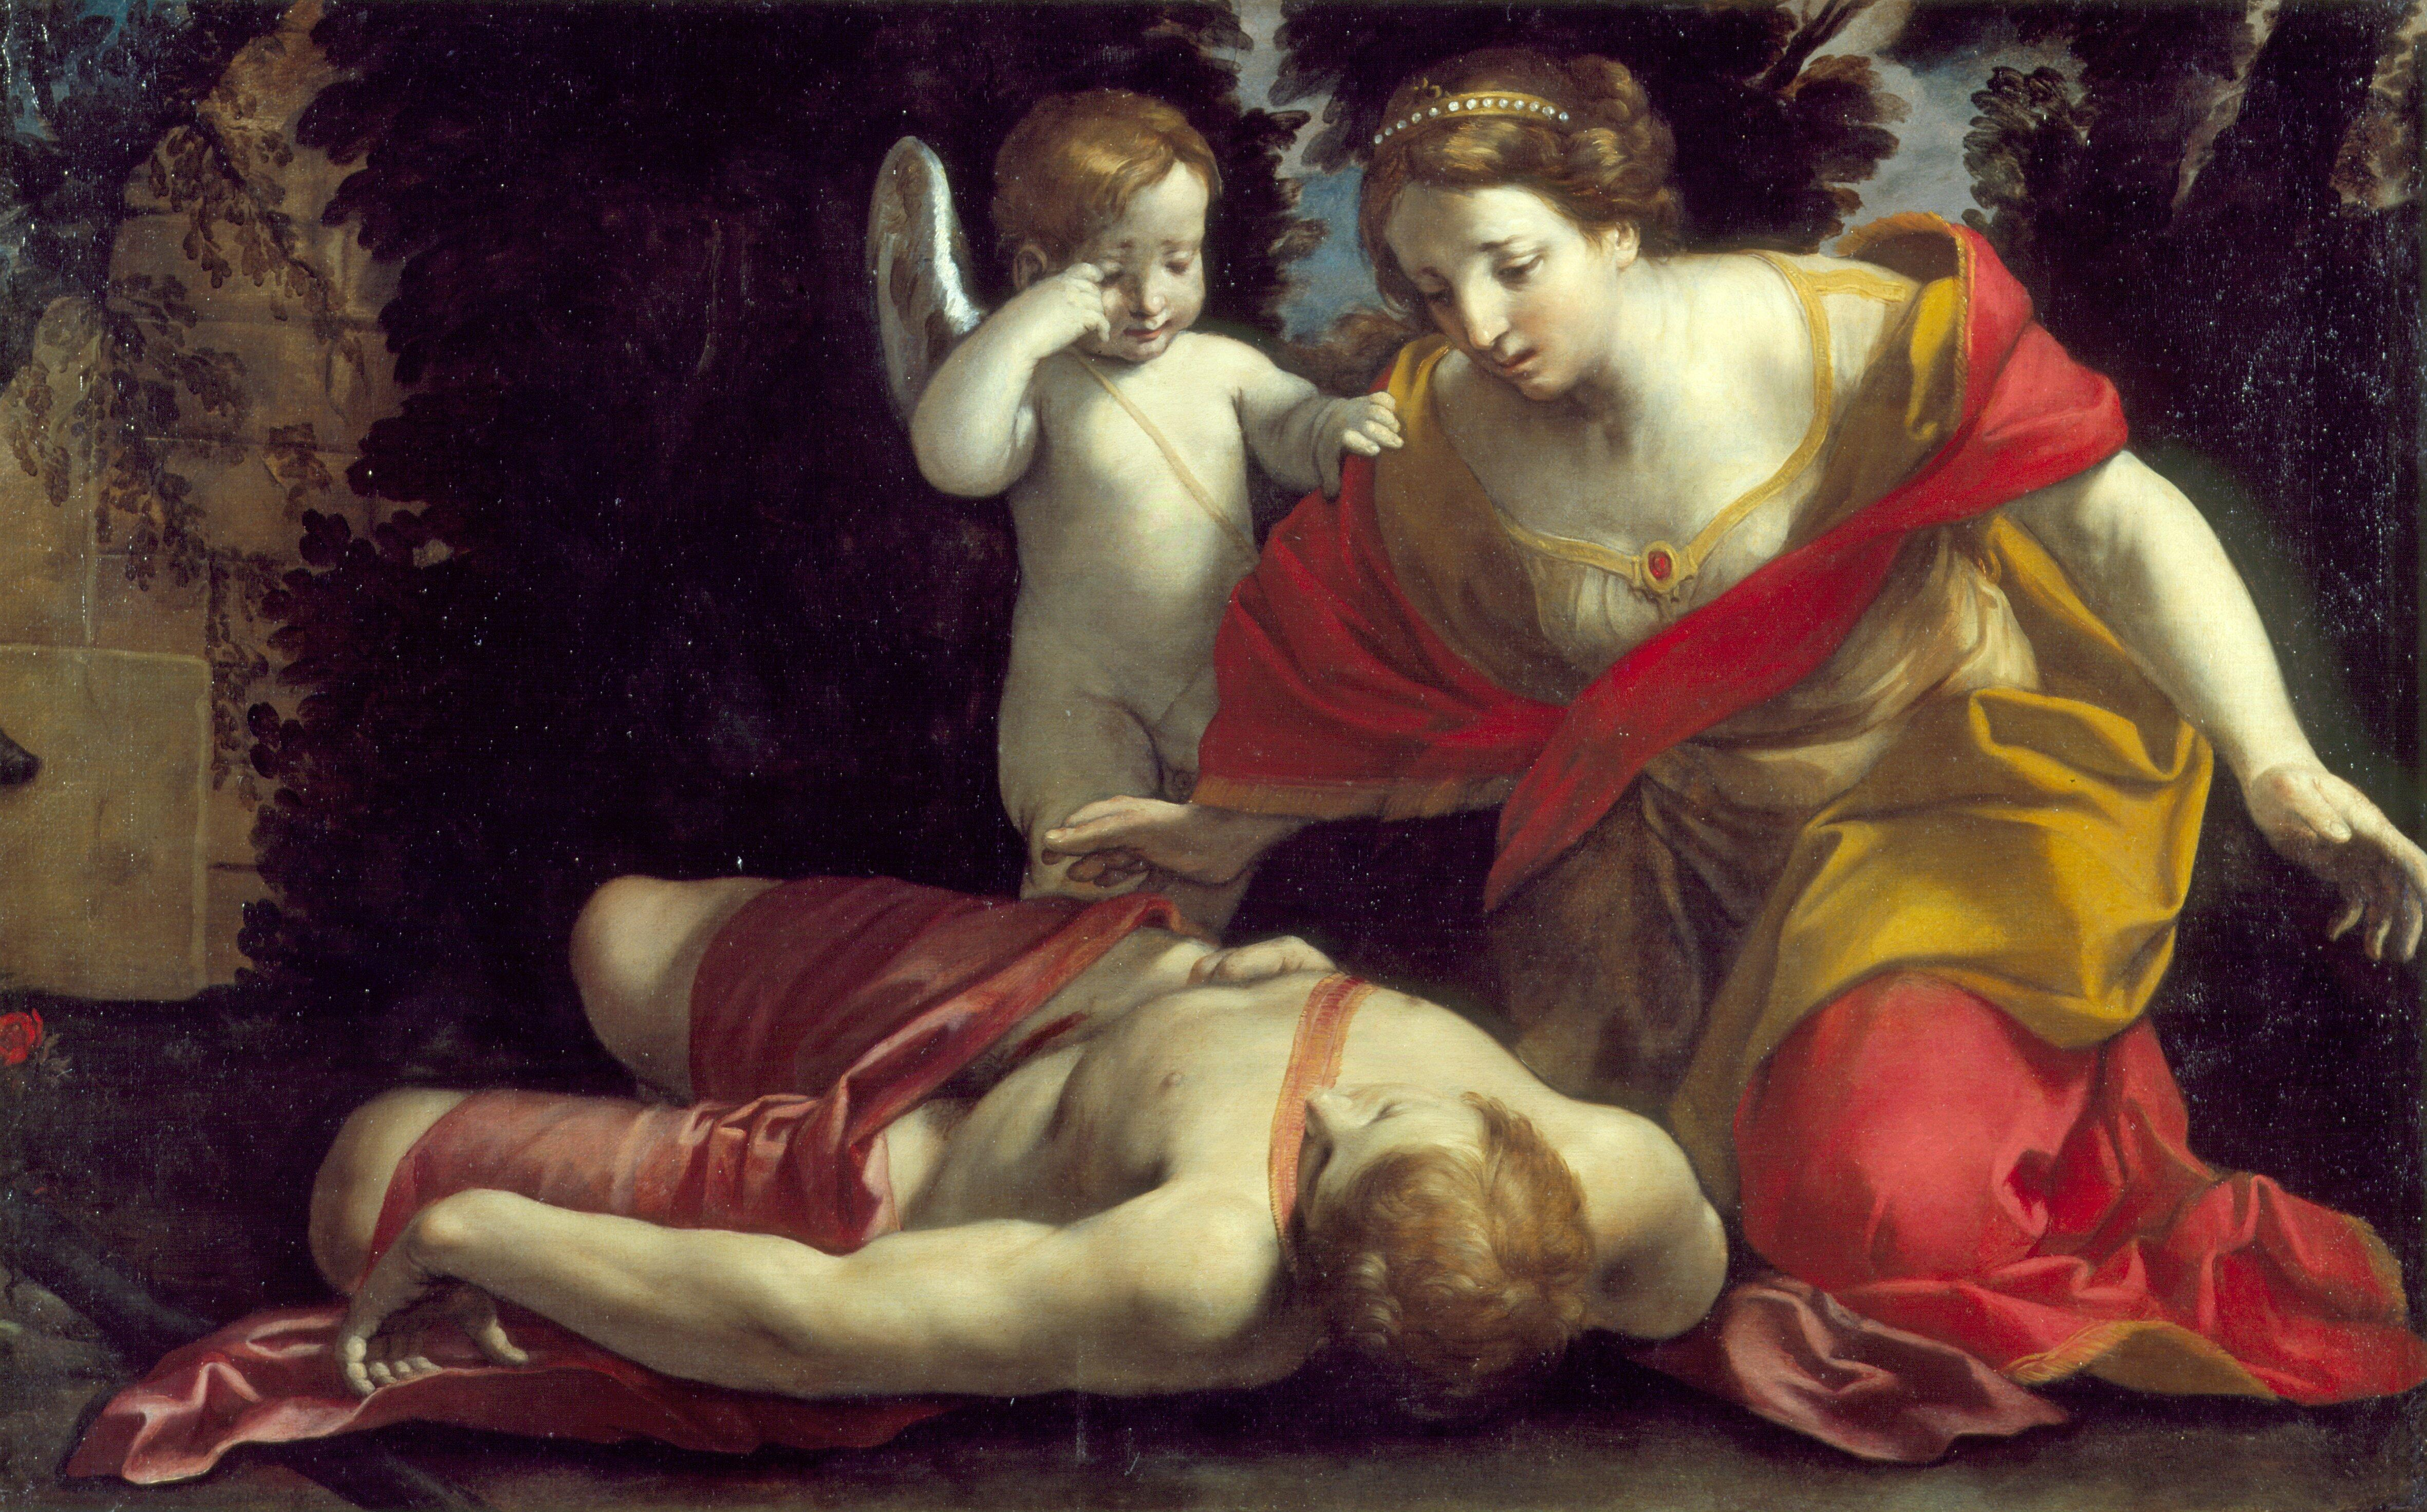
\includegraphics[scale=0.07]{Gessi_Giovan_Francesco-Morte_di_Adone.jpg}}
			};
		\end{tikzpicture}
	\end{figure}
	
	\begin{minipage}{\linewidth}
		\centering
		\begin{tikzpicture}
			\node[draw,dashed]
			{
				\fboxrule=4pt
				\fcolorbox{white}{white}{
					\fbox{
						\begin{minipage}{60mm}
							\raggedright
							{
								La tela raffigura una donna addolorata, in posizione inginocchiata davanti al corpo supino in primo piano di un bellissimo uomo seminudo che rappresenta Adone; vicino alla donna che ama il protagonista del dipinto è posto un amorino piangente che porta la manina ad un occhio. Nascosto nell'angolo a sinistra appare il muso del cinghiale che ha ucciso Adone durante la sua battuta di caccia.
							}
						\end{minipage}
					}
				}
			};
		\end{tikzpicture}
	\end{minipage}

	\section{Fonte della descrizioni}
	Tutte le descrizioni riportate prendono spunto dalle descrizioni delle opere all'interno del sito \href{http://webapp.comune.pesaro.pu.it/scriptcase/app/pandora/treemenu/}{\textcolor{blue}{Pandora}}
	
	\vspace*{\fill}
	% Print license shield
	\doclicenseThis
	
	\newpage
	%-------- End image --------
		
	
	
\end{document}